\documentclass[12pt,oneside,reqno]{ta-its}
\usepackage{hyperref}
\usepackage{listings}
\usepackage{float}
\usepackage{mdframed}
\usepackage{wrapfig}

\renewcommand{\lstlistingname}{Kode Sumber}
\renewcommand{\lstlistlistingname}{DAFTAR KODE SUMBER}

\title{Implementasi \textit{Headless Browser} untuk \textit{Load Testing} Berbasis \textit{Web Service} Menggunakan Infrastruktur \textit{Docker}
}{Headless Browser Implementation for Load Testing Based on Web Service Using Docker Infrastructure}{IF184802}

\author{Cahya Putra Hikmawan}{05111540000119}

\supervisorOne{Royyana Muslim Ijtihadie, S.Kom., M.Kom., Ph.D.}{197708242003041001}
\supervisorTwo{Bagus Jati Santoso, S.Kom., Ph.D.}{198611252018031001}

\degree{Sarjana Komputer}{Arsitektur dan Jaringan Komputer}{S1}{Informatika}{Informatics}{Teknologi Informasi dan Komunikasi}{FTIK-ITS}{Information Technology and Communication}

\time{Juni}{2019}

\begin{document}
	\frontmatter % Halaman dengan penomoran romawi kecil
	\maketitle
	\legalityPaper % Lembar Pengesahan
	
    \begin{abstrak}
		Saat ini pengembangan aplikasi berbasis web sangat banyak dilakukan. Dalam pengembangan web, akan diperlukan uji beban yang dilakukan pada web yang dikembangkan sebelum diluncurkan ke tahap produksi. Dilakukannya uji beban tentu saja untuk menghindari terjadinya kegagalan muat ketika sudah diluncurkan.
		
		\indent Dalam melakukan uji beban, pengembang akan membutuhkan resource user untuk mengakses web dan waktu yang cukup lama karena dilakukan secara manual. Beberapa contoh tools yang dapat mengatasi hal tersebut untuk melakukan uji beban yaitu JMeter, k6 dan sebagainya. Namun tools tersebut menggunakan thread untuk resource user-nya, bila dilihat kondisi lapangan yaitu pengguna mengakses web menggunakan browser dan memiliki IP masing-masing, thread kurang bisa mengatasi hal tersebut. Oleh karena itu, dibutuhkan tools yang dapat menangani hal tersebut, salah satunya yaitu pengujian secara headless yang memanfaatkan infrastruktur Docker dan melakukan otomasi untuk pengambilan data uji beban. Docker akan menjadi resource user yang mengakses melalui headless browser untuk uji beban.
		
		\indent Pada tugas akhir ini, dibuat sistem yang mampu melayani uji beban pada suatu web. Dengan menggunakan Docker Container sebagai load generator yang akan bisa melakukan akses ke web yang diuji melalui Headless Chrome dan akan dilakukan otomasi pengambilan data uji beban menggunakan API Puppeteer. Selain itu, sistem juga dilengkapi task scheduler untuk melayani permintaan uji beban dari multiuser. Hasil uji yang didapatkan pada sistem ini adalah beberapa performance metrics, error console pada browser dan tangkapan layar terhadap interface web yang diuji.
		
		\indent Hasil uji coba menunjukkan bahwa Docker Container dapat dijadikan sebagai resource user karena sumberdaya yang dibutuhkan hanya 1,3MB setiap Docker Container dalam keadaan sleep, namun untuk ketika Puppeteer mengakses web yang diuji melalui Headless Chrome membutuhkan sumberdaya CPU dan RAM yang cukup tinggi jika dijalankan secara bersama-sama. Maka dari itu, dibutuhkan pembatasan atau manajemen proses untuk Headless Chrome. Sedangkan untuk data uji beban yang dihasilkan dari Headless Chrome sangat memuaskan. \\

	\noindent \textbf{Kata-Kunci}: headless browser, headless chrome, load test, puppeteer, docker
\end{abstrak}

\newpage
\begin{abstract}
		Nowadays web-based application development is very much done. In web development, a load test will be needed on the web that was developed before being launched into the production stage. The load test is carried out of course to avoid loading failure when it is launched.
		
		\indent In carrying out load tests, developers will need a resource user to access the web and a considerable amount of time because it is done manually. Some examples of tools that can overcome this are to carry out load tests namely JMeter, k6 and so on. However, these tools use threads for their resource users, if you see field conditions, that is, users access the web using a browser and have their own IP, the thread is less able to overcome this. Therefore, we need tools that can handle this, one of which is headless testing that utilizes Docker infrastructure and automates the load test data collection. Docker will be a resource user who accesses through the headless browser for load testing.
		
		\indent In this final project, a system that is capable of serving load tests on a web is made. By using Docker Container as a load generator that will be able to access the web tested through Headless Chrome and automation of load test data retrieval will be carried out using the Puppeteer API. In addition, the system also features a task scheduler to serve multiuser load test requests. The test results obtained in this system are several performance metrics, browser console errors and screenshots of the tested web interface.
		
		\indent The trial results show that Docker Container can be used as a resource user because the resources needed are only 1.3MB per Docker Container in a sleep state, but for when Puppeteer accesses the web tested through Headless Chrome it requires high CPU and RAM resources if run together -same. Therefore, restrictions or process management are needed for Headless Chrome. Whereas for load test data generated from Headless Chrome is very satisfying. \\		

	\noindent \textbf{Keywords}: headless browser, headless chrome, load test, puppeteer, docker
\end{abstract}
	\chapter{KATA PENGANTAR}
		Bismillahirrahmanirrahim, \\
		Alhamdulillahirabbil’alamin, segala puji bagi Allah SWT yang telah melimpahkan rahmat dan hidayah-Nya sehingga penulis dapat menyelesaikan Tugas Akhir yang berjudul "\textbf{Implementasi \textit{Headless Browser} untuk \textit{Load Testing} Berbasis \textit{Web Service} Menggunakan Infrastruktur \textit{Docker}}". Pengerjaan Tugas Akhir ini merupakan kesempatan yang baik bagi penulis untuk belajar lebih banyak, serta memperdalam apa yang telah didapatkan penulis selama menempuh perkuliahan di Informatika ITS. Dengan adanya Tugas Akhir ini, penulis juga dapat menghasilkan suatu implementasi dari apa yang penulis pelajari. Sehingga penulis mengharapkan implementasi Tugas Akhir ini dapat memberikan kontribusi dan manfaat. Selesainya Tugas Akhir ini tidak lepas dari bantuan dan dukungan dari beberapa pihak baik langsung maupun tidak langsung. Sehingga pada kesempatan ini penulis mengucapkan terima kasih kepada:
		\begin{enumerate}
			\item Allah SWT atas anugerah-Nya yang tidak terkira dan Nabi Muhammad SAW.
			\item Ibu dan Ayah yang selalu memberikan doa yang tak terhingga, dukungan moral dan material selama penulis hidup. Serta selalu memberi semangat dan dorongan untuk menyelesaikan Tugas Akhir ini.
			\item Bapak Royyana Muslim Ijtihadie, S.Kom, M.Kom, Ph.D., selaku pembimbing I dan Bapak Bagus Jati Santoso, S.Kom., Ph.D., selaku dosen pembimbing II yang telah membantu, membimbing dan memotivasi penulis mulai dari pengerjaan proposal hingga terselesaikannya Tugas Akhir ini.
			\item Bapak Darlis Herumurti, S.Kom., M.Kom., selaku Kepala Jurusan Teknik Informatika ITS saat ini, Bapak Radityo Anggoro, S.Kom., M.Sc., selaku koordinator TA dan segenap dosen dan karyawan Teknik Informatika yang telah memberikan ilmu dan pengalamannya, serta memberikan fasilitas yang aman dan nyaman, sehingga penulis dapat menempuh studi di Informatika ITS.
			\item Seluruh teman-teman Laboratorium Arsitektur dan Jaringan Komputer (AJK): Putol, Sinyo, Penyok, Satria, Nahda, Hana, Daus, Aguel, Raldo, Tamtam, Khawari, Haura, Lia, Sulton, Fawwaz, Yoga dan Mail yang bersedia direpotkan, merepotkan dan menemani penulis dalam mengerjakan Tugas Akhir.
			\item Alumni-alumni AJK, Mas Daniel, Mas Uul, Mas Wicak, Asbun, Toni, Pak Lek, Mas Fatih, Mbak Nindy dan Mbak Zaza yang selalu membuat saya termotivasi untuk lulus dan memberikan arahan dalam pengerjaan Tugas Akhir ini.
			\item Rozana Firdausi yang selalu merepotkan, direpotkan, menemani dan memberikan semangat secara langsung dan tidak langsung, sehingga penulis dapat mengerjakan Tugas Akhir ini dengan baik.
			\item Tim Proyek Arya Fajar Production, Pak Arya Yudhi Wijaya, S.Kom, M.Kom., Pak Fajar Baskoro, S.Kom., MT., Pak Ary Mazharuddin S., S.Kom., M.Comp.Sc., Mas Jumali, Tayar, Sinyo, Fajri, Adit, Irsa, Tamtam, Fasma, Jonathan, Nila, Andhika dan Fawwaz yang telah merepotkan dan memberikan pengalaman yang berharga bagi penulis dalam hal lapangan pekerjaan secara nyata.
			\item Grup Sayang: Sinyo, Yoza, Tayar, Fajri, Yayan, Alvin, Bas, Putol, Chasni, Raca dan reza yang telah memberikan secuil motivasi dan memberikan dampak yang baik secara jasmani maupun secara rohani penulis.
			\item Teman-teman satu bimbingan, Hero, Didin, Satria dan Nahda yang telah sama-sama berjuang dalam mengerjakan dan mengimplementasikan Tugas Akhir tentang Sistem Terdistribusi dan Komputasi Awan.
			\item Teman-teman angkatan 2015 yang menemani dari awal hingga akhir serta semua pihak yang turut membantu penulis dalam menyelesaikan Tugas Akhir ini.
		\end{enumerate}
		
		
		\indent Penulis sangat menyadari bahwa Tugas Akhir ini masih memiliki banyak kekurangan. Sehingga penulis memohon maaf secara tulus kepada pembaca. Dengan kerendahan hati, penulis mengharapkan kritik dan saran yang membangun dari pembaca sebagai pembelajaran dan perbaikan untuk kedepannya. \\

		\hfill Surabaya, Juni 2019 \\ \\
		
		\hfill Cahya Putra Hikmawan

	\cleardoublepage % Mengisi penanda halaman genap yang kosong

	\tableofcontents % Daftar Isi
	\listoftables % Daftar Tabel
	\listoffigures % Daftar Gambar
	\lstlistoflistings % Daftar Kode Sumber

	\mainmatter
	\chapter{PENDAHULUAN}
	Pada bab ini akan dipaparkan mengenai garis besar tugas akhir yang meliputi latar belakang, tujuan, rumusan dan batasan permasalahan, metodologi pembuatan tugas akhir, dan sistematika penulisan.
        
	\section{Latar Belakang}
		Saat ini pengembangan aplikasi berbasis web sangat banyak dilakukan. Dalam pengembangan web, akan diperlukan uji beban yang dilakukan pada web yang dikembangkan sebelum diluncurkan ke tahap produksi. Salah satu teknik uji beban adalah \textit{Headless Testing}, salah satu \textit{browser} yang menggunakan teknik ini adalah \textit{Headless Chrome}. Teknik ini menyediakan akses kontrol seperti \textit{browser} pada umumnya untuk mendapatkan data dokumen uji beban, hanya saja teknik ini berjalan secara \textit{headless} atau tanpa menampilkan antarmuka pengguna. Dikarenakan berjalan secara \textit{headless}, maka untuk melakukan pengambilan data dokumen uji beban dilakukan menggunakan baris perintah atau \textit{CLI(Command Line Interface)}.
		
		\indent Pengembang aplikasi web tentu saja membutuhkan teknik untuk uji beban, namun dalam melakukan uji beban dibutuhkan \textit{resource user} untuk mengakses web dan waktu yang cukup lama karena dilakukan secara manual. Oleh karena itu, dibutuhkan suatu sistem yang dapat melakukan otomasi untuk uji beban web, membuat \textit{load generator} yang digunakan sebagai \textit{resource user} dan dapat mempersingkat waktu uji beban.
		
		\indent Pada tugas akhir ini, akan dibangun sebuah sistem uji beban menggunakan teknik secara \textit{headless} yang akan memanfaatkan \textit{Headless Chrome} sebagai \textit{tester} dan membuat \textit{load generator} yang memanfaatkan infrastruktur \textit{Docker} sebagai \textit{resource user}, serta otomasi pengambilan data dari \textit{tester} menggunakan pustaka \textit{Node} yaitu \textit{Puppeteer}\cite{puppeteer}.

	\section{Rumusan Masalah}
       	Rumusan masalah yang diangkat dalam tugas akhir ini dapat dipaparkan sebagai berikut :
		\begin{enumerate}
			\item Bagaimana cara mengimplementasikan \textit{Headless Chrome} sebagai \textit{tester} untuk \textit{load generator}?
			\item Bagaimana cara mengimplementasikan \textit{Docker} bisa menjadi \textit{load generator} untuk uji beban?
			\item Bagaimana cara menghasilkan laporan uji beban pada web?
			\item Bagaimana mengelola layanan pengujian untuk \textit{multiuser} dalam bentuk antrian?
		\end{enumerate}

	\section{Batasan Masalah}
		Dari permasalahan yang telah dipaparkan di atas, terdapat beberapa batasan masalah pada tugas akhir ini, yaitu:
		\begin{enumerate}
			\item \textit{Headless Browser} yang digunakan adalah \textit{Headless Chrome}.
			\item Kontainer yang digunakan adalah \textit{Docker}.
			\item Distribusi kontainer menggunakan \textit{Docker Swarm}.
			\item Aplikasi yang akan diuji berupa aplikasi web.
			\item Uji coba aplikasi akan menggunakan  \textit{Node library yang menyediakan API (Application Programming Interface)} untuk mengontrol \textit{Headless Chrome} yaitu \textit{Puppeteer}.
		\end{enumerate}

	\section{Tujuan}
       	Tujuan pembuatan tugas akhir ini antara lain:
       	\begin{enumerate}
       		\item Membuat sistem manajemen pengujian aplikasi secara \textit{headless} menggunakan \textit{Headless Chrome}.
       		\item Membuat sistem agar \textit{Docker} bisa menjadi \textit{load generator} untuk pengujian.
       		\item Membuat sistem untuk menampilkan laporan uji beban pada web.
       		\item Membuat sistem yang dapat mengelola permintaan layanan uji beban dari \textit{multiuser} berupa antrian.
       	\end{enumerate}
        
	\section{Manfaat}
		Manfaat dari pembuatan tugas akhir ini yaitu:
		\begin{enumerate}
			\item Mempelajari penggunaan \textit{Headless Browser} untuk pengujian suatu aplikasi yaitu \textit{Headless Chrome}
			\item Mempelajadi penggunaan \textit{Docker} sebagai \textit{load generator} untuk melakukan uji beban.
			\item Mengetahui performa uji beban suatu aplikasi web.
			\item Meminimalisir adanya kegagalan web saat dimuat ketika sudah diluncurkan.
		\end{enumerate}
	
	\section{Metodologi}
		Metodologi yang digunakan untuk pembuatan Tugas Akhir ini adalah sebagai berikut:	
		\subsection{Penyusunan Proposal Tugas Akhir}
			Proposal tugas akhir ini berisi tentang deskripsi pendahuluan dari tugas
			akhir yang akan dibuat. Pendahuluan ini terdiri dari hal yang menjadi latar
			belakang diajukannya usulan tugas akhir, rumusan masalah yang diangkat,
			batasan masalah untuk tugas akhir, tujuan dari pembuatan tugas akhir, dan
			manfaat dari hasil pembuatan tugas akhir. Selain itu dijabarkan pula tinjauan
			pustaka yang digunakan sebagai referensi pendukung pembuatan tugas akhir.
			Sub bab metodologi berisi penjelasan mengenai tahapan penyusunan tugas
			akhir mulai dari penyusunan proposal hingga penyusunan buku tugas akhir.
			Terdapat pula sub bab jadwal kegiatan yang menjelaskan jadwal pengerjaan
			tugas akhir.	
		\subsection{Studi Literatur}
			Pada tahap ini dilakukan pencarian informasi dan referensi mengenai \textit{Headless Chrome}, \textit{Puppeteer} dan \textit{Docker} untuk mendukung dan memastikan setiap tahap pembuatan tugas akhir sesuai dengan standar dan konsep yang berlaku, serta dapat diimplementasikan. Sumber informasi dan referensi bisa didapatkan dari buku, jurnal dan internet.
		\subsection{Analisis dan Desain Perangkat Lunak}
			Pada tahap ini dilakukan analisis dan perancangan terhadap arsitektur sistem yang akan dibuat. Tahap ini merupakan tahap yang paling penting dimana segala bentuk implementasi bisa bekerja dengan baik ketika arsitektur sistem yang baik pula.
		\subsection{Implementasi Perangkat Lunak}
			Pada tahap ini dilakukan implementasi atau realisasi dari hasil analisis dan perancangan arsitektur yang sudah dibuat sebelumnya, sehingga menjadi sebuah infrastruktur yang sesuai dengan apa yang direncanakan. 
		\subsection{Pengujian dan Evaluasi}
			Pada tahap ini dilakukan pengujian untuk mengukur performa web dan kegagalan saat dimuat menggunakan arsitektur sistem yang sudah dibuat menggunakan infrastruktur \textit{Docker}. Beberapa performa yang diukur pada pengujian antara lain, \textit{Load Event End}, \textit{Response End}, \textit{First Meaningful Paint}, \textit{CSS Tracing End} dan \textit{Dom Content Loaded} dalam satuan \textit{ms(millisecond)} serta \textit{error console}. Setelah dilakukan uji coba, maka dilakukan evaluasi terhadap kinerja arsitektur sistem yang telah diimplementasikan dengan harapan bisa diperbaiki ketika ada pengembangan ke depannya.
		\subsection{Penyusunan Buku Tugas Akhir}
			Pada tahap ini dilakukan penyusunan buku tugas akhir yang berisikan dokumentasi yang mencakup teori, konsep, implementasi dan hasil pengerjaan tugas akhir.
	
	\section{Sistematika Penulisan}
		Sistematika penulisan laporan tugas akhir secara garis besar adalah sebagai berikut:
		\begin{enumerate}
			\item Bab I. Pendahuluan\\
				Bab ini berisi penjelasan mengenai latar belakang, rumusan masalah, batasan masalah, tujuan, manfaat, metodologi dan sistematika penulisan dari pembuatan tugas akhir.
			\item Bab II. Tinjauan Pustaka\\
				Bab ini berisi kajian teori atau penjelasan metode, algoritme, \textit{library} dan \textit{tools} yang digunakan dalam penyusunan tugas akhir ini. Kajian teori yang dimaksud berisi tentang penjelasan singkat mengenai \textit{Headless Browser}, \textit{Headless Chrome}, \textit{Puppeteer}, \textit{NodeJS}, \textit{Docker}, \textit{Docker Swarm}, \textit{Laravel} dan \textit{Python}.
			\item Bab III. Desain dan Perancangan\\
				Bab ini berisi mengenai analisis dan perancangan arsitektur sistem yang akan diimplementasikan pada tugas akhir ini.
			\item Bab IV. Implementasi\\
				Bab ini berisi bahasan tentang implementasi dari arsitektur sistem yang dibuat pada bab sebelumnya. Penjelasan berupa kode program yang digunakan untuk mengimplementasikan sistem.
			\item Bab V. Pengujian dan Evaluasi\\
				Bab ini berisi bahasan tentang tahapan uji coba terhadap performa web dan evaluasi terhadap sistem yang dibuat.
			\item Bab VI. Penutup\\
				Bab ini merupakan bab terakhir yang memaparkan kesimpulan dari hasil pengujian dan evaluasi yang telah dilakukan. Pada bab ini juga terdapat saran yang ditujukan bagi pembaca yang berminat untuk melakukan pengembangan lebih lanjut.
			\item Daftar Pustaka\\
				Bab ini berisi daftar pustaka yang dijadikan literatur dalam tugas akhir.
			\item Lampiran\\
				Dalam lampiran terdapat kode sumber program secara keseluruhan.
		\end{enumerate}
	\chapter{TINJAUAN PUSTAKA}
	\section{\textit{Headless Browser}}
		\textit{Headless Browser} merupakan jenis perangkat lunak yang dapat mengakses halaman web, namun tidak menampilkan antarmuka pengguna. Seperti peramban pada umumnya, \textit{Headless Browser} juga memiliki kemampuan yang sama, hanya saja menyisakan mesin dan lingkungan \textit{javascript}. Oleh karena itu \textit{Headless Browser} hanya bisa diakses menggunakan baris perintah atau \textit{CLI(Command Line Interface)}\cite{headless_browser}. Beberapa \textit{Headless Browser} yaitu \textit{Headless Chrome}, \textit{Selenium WebDriver} dan \textit{Firefox Headless Mode}. Salah satu \textit{Headless Browser} yang akan digunakan pada Tugas Akhir ini adalah \textit{Headless Chrome}, karena \textit{Headless Chrome} memiliki fitur khusus yang bisa ditemukan pada bagian \textit{performance}. \textit{Headless Chrome} juga memiliki fitur umum seperti \textit{Headless Browser} yang lain. Beberapa fitur umumnya yaitu\cite{headless_browser_2}:
		
		\begin{enumerate}
			\item Memudahkan untuk melakukan pengujian secara otomatis.
			\item Bisa dijalankan di server, mode \textit{headless} tidak membutuhkan antarmuka pengguna.
			\item Membuat dokumen atau file seperti PDF dan Screenshot.
			\item \textit{Debugging}.\\
		\end{enumerate}

		\indent Dalam tugas akhir ini, \textit{Headless Browser} akan digunakan sebagai browser untuk menguji web yang akan diuji performanya, sedangkan jenis yang digunakan adalah \textit{Headless Chrome}. \textit{Headless Chrome} saat ini dikembangkan oleh \textit{Google Developer} dan memiliki lisensi dari \textit{Apache 2.0 License}.
			
	\section{\textit{Node.js}}
		\textit{Node.js} atau \textit{node} adalah sebuah platform dengan lingkungan \textit{JavaScript} sisi server.\textit{ Node.js} berbasis pada \textit{Chrome's JavaScript Runtime} yang menggunakan teknologi V8 dan berfokus pada performa maupun konsumsi memori rendah. Tapi V8 juga mendukung proses server yang berjalan lama. Tidak seperti kebanyakan platform modern yang lain dengan mengandalkan \textit{multithreading}. \textit{Node.js} menggunakan penjadwalan I/O secara asinkron. Proses pada \textit{Node.js} dibayangkan sebagai proses \textit{single-threaded daemon}. Hal ini berbeda dengan kebanyakan sistem penjadwalan dalam bahasa pemrograman lain yang berbentuk \textit{library}. \textit{Node.js} seringkali digunakan pengembang sebagai web server atau layanan \textit{API}. Selain itu \textit{Node.js} juga mendukung \textit{event callback} untuk setiap penggunaan fungsi, memungkinkan ketika fungsi tersebut dipanggil akan terjadi \textit{sleep} ketika tidak ada hasil apapun.\cite{nodejs}\cite{nodejs_2}.
		
	 	\indent Salah satu pustaka \textit{Node.js} yang menyediakan layanan \textit{API} adalah \textit{Puppeteer}. Pada tugas akhir ini, \textit{Node.js} akan digunakan sebagai bahasa pemrograman untuk mengimplementasikan \textit{Puppeteer}.
		
		\subsection{\textit{Puppeteer}}
			\textit{Puppeteer} adalah sebuah pustaka dari \textit{Node} yang memiliki kemampuan yang mumpuni untuk memberikan layanan \textit{API} yang berfungsi untuk mengontrol layanan dari \textit{Chrome} atau \textit{Chromium}. Selain itu, kemampuan kontrol \textit{Puppeteer} sangat memungkinkan untuk akses pada protokol \textit{Devtools Protocol} yang saat ini dikembangkan oleh tim \textit{Google Developer}, dimana protokol tersebut memiliki kemampuan yang cukup berguna yaitu sebagai \textit{tools instrument}, \textit{inspect}, \textit{debug}, dan \textit{profile chrome}.\cite{puppeteer} \\
			\indent Dibandingkan dengan \textit{PhantomJS} yang sudah tidak dikembangkan lagi, \textit{Puppeteer} masih dikembangkan secara berkala. Begitupun fitur-fitur yang disediakan \textit{Puppeteer} sangat mumpuni untuk melakukan beberapa pengujian terhadap web yaitu melakukan pengambilan gambar ataupun pdf, otomasi, pengujian antarmuka pengguna, \textit{keyboard input}, \textit{timeline trace} untuk mendapatkan performa dan ekstensi pada \textit{Chrome}. Untuk lebih jelasnya struktur diagram \textit{Puppeteer} ditunjukkan pada Gambar \ref{puppeteeroverview}.
			\begin{figure}[H]
				\centering
				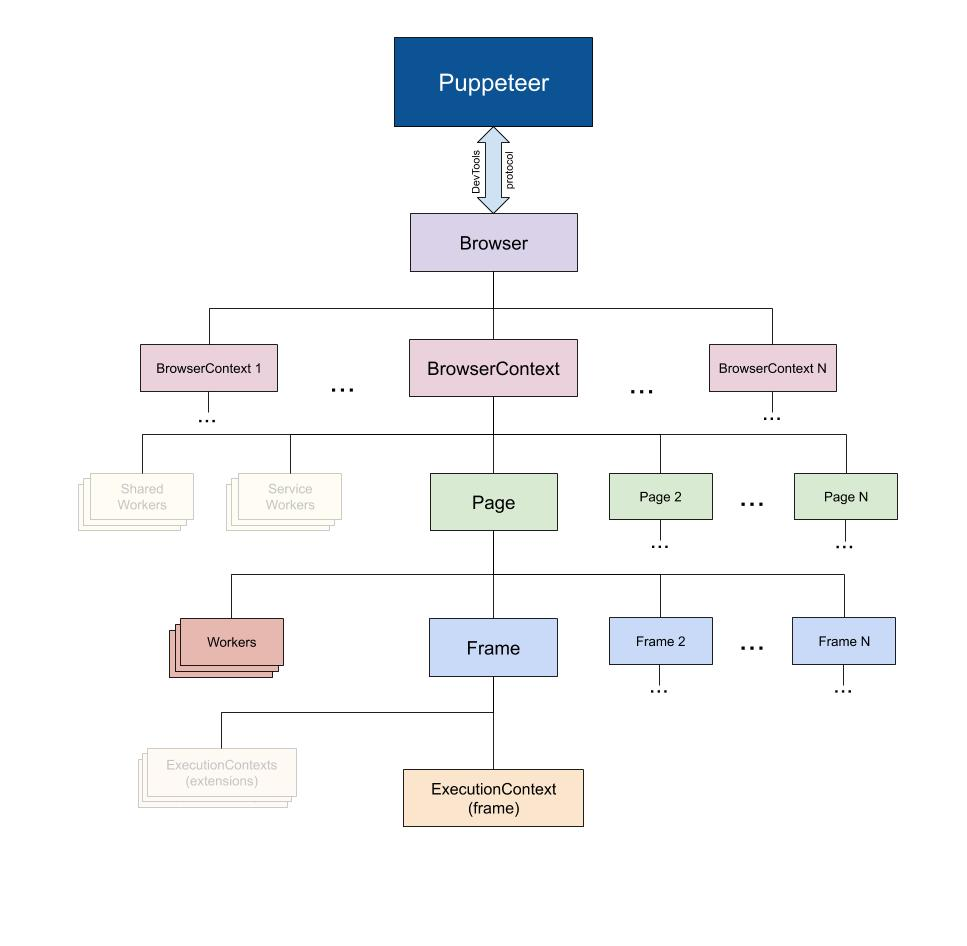
\includegraphics[width=9cm,height=10cm]{Images/C-2/puppeteeroverview.jpg}
				\caption{Struktur diagram \textit{Puppeteer}}
				\label{puppeteeroverview}
			\end{figure}
			
			\indent Pada tugas akhir ini, \textit{Puppeteer} akan digunakan sebagai alat untuk mengontrol \textit{Headless Browser} yang akan diimplementasikan pada sistem perangkat lunak yang akan dibangun, karena lebih mumpuni dan memiliki beragam fitur \textit{API} untuk mengakses \textit{Headless Chrome} dibandingkan dengan pustaka \textit{Node} yang lain.
		
	\section{\textit{Docker}}
		\textit{Docker} adalah sebuah platform terbuka yang berfungsi sebagai wadah untuk membangun, membungkus, dan menjalankan aplikasi supaya dapat berfungsi sebagaimana mestinya. \textit{Docker} memungkinkan untuk memisahkankan aplikasi dari infrastruktur supaya \textit{software} dapat di jalankan dengan lebih cepat. \textit{Docker} pada dasarnya memperluas \textit{LXC(Linux Containers)} menggunakan kernel dan \textit{API} pada level aplikasi yang akan dijalankan secara bersamaan pada isolasi \textit{CPU}, memori, I/O, jaringan dan yang lainnya. \textit{Docker} juga menggunakan \textit{namespaces} untuk mengisolasi segala tampilan pada aplikasi yang mendasari lingkungan operasinya, termasuk \textit{process tree}, jaringan, ID pengguna, dan file sistem. 
		
		\indent \textit{Docker Container} dibuat oleh sebuah \textit{Docker Images}. \textit{Docker Images} hanya mencakup dasar dari operasi sistem atau hanya memuat set dari \textit{prebuilt} aplikasi yang sudah siap dijalankan. Ketika membuat \textit{Docker Images}, bisa menjalankan perintah (yaitu apt-get install) membentuk lapisan baru diatas lapisan sebelumnya. Perintah tersebut bisa dijalankan manual satu-persatu atau secara otomatis menggunakan \textit{Dockerfile}. 
		
		\indent Setiap \textit{Dockerfile} adalah kombinasi beberapa perintah yang dibuat menjadi menjadi satu atau \textit{script} yang bisa dijalankan secara otomatis sebagai \textit{Docker Images} utama atau untuk membuat \textit{Docker Images} yang baru\cite{docker}\cite{docker_2}. \textit{Docker} juga menyediakan layanan untuk mengunduh dan mengupload \textit{Docker images} melalui \texttt{https://hub.docker.com/}. Untuk melihat perbedaan antara kontainer dan \textit{VM(Virtual Machine)} dapat dilihat pada Gambar \ref{containervm}.
	
		\indent Pada tugas akhir ini, \textit{Docker Container} akan digunakan sebagai pengguna untuk mengakses web yang akan diuji, dan bisa diumpamakan sebagai pengguna asli untuk otomasi pengujiannya. \\
		
		\begin{figure}[H]
			\centering
			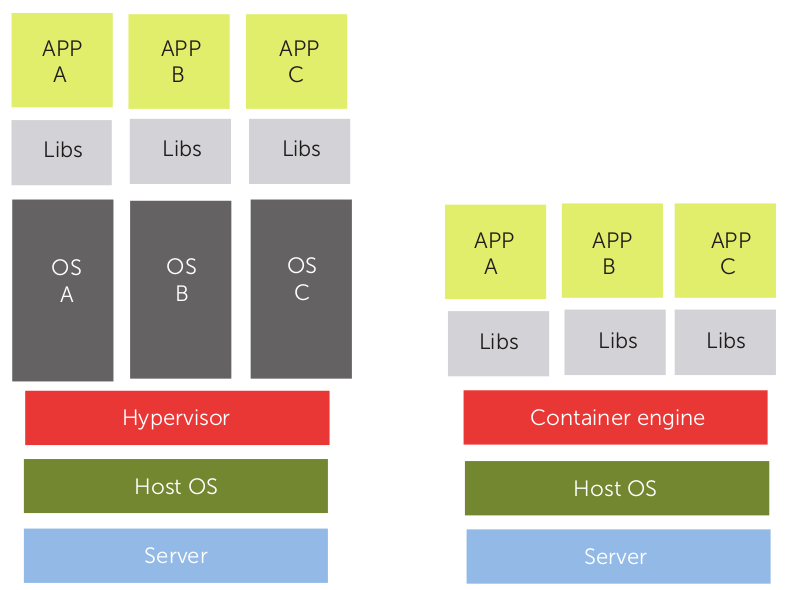
\includegraphics[width=9cm,height=7cm]{Images/C-2/containervm.png}
			\caption{Perbandingan kontainer dan \textit{Virtual Machine}\cite{docker_2}}
			\label{containervm}
		\end{figure}
	
		\subsection{\textit{Docker Swarm}}
			\textit{Docker Swarm} - disebut juga \textit{Swarm} adalah mode pada \textit{Docker} yang memiliki fitur yang tertanam pada mesinnya untuk Manajemen \textit{Cluster} atau \textit{Orkestrasi}. Pada mode \textit{Swarm} akan terdapat lebih dari satu \textit{host} dimana \textit{host} tersebut bisa berfungsi sebagai manager, worker, atau bisa juga keduanya. Konsep pada \textit{Swarm} antara lain adalah \textit{Nodes}, \textit{Services}, \textit{Tasks} dan \textit{Load Balancing}. Mode \textit{Swarm} juga memudahkan untuk mengatur bagian replikasi, jaringan, penyimpanan, port dan sebagainya.
			
			\indent Dibandingkan dengan kontainer yang berdiri sendiri, \textit{Swarm} lebih mudah untuk mengubah konfigurasi servis, termasuk penyimpanan dan jaringannya tanpa harus menyalakan kembali kontainer secara manual. \textit{Docker} akan otomatis memperbarui konfigurasi dengan cara menghentikan \textit{service task} yang memiliki konfigurasi lama, kemudian akan membuat kembali \textit{service task} menggunakan konfigurasi yang sudah diperbarui. \textit{Swarm} juga bisa menggunakan \textit{Docker Compose} untuk mendefinisikan dan menjalankan kontainer, \textit{Docker Compose} menggunakan \textit{YAML file} sebagai konfigurasinya.\cite{docker_swarm}.
			
			\indent Pada saat mode \textit{Swarm}, \textit{node manager} akan mengimplementasikan \textit{Raft Consensus Algorithm} untuk memanajemen \textit{cluster}. \textit{Consensus} memungkinan manajer untuk mengatur dan menjadwal \textit{tasks} pada setiap \textit{cluster} dan memastikan status tetap konsisten, dimana ketika ada salah satu \textit{nodes} yang gagal dalam mejalankan servis, manajer bisa mengembalikan servis menjadi stabil kembali\cite{docker_swarm_raft}. Untuk melihat rute diagram ketika mode \textit{Swarm} dapat dilihat pada Gambar \ref{swarmdiagramroute}.
			
			\begin{figure}[H]
				\centering
				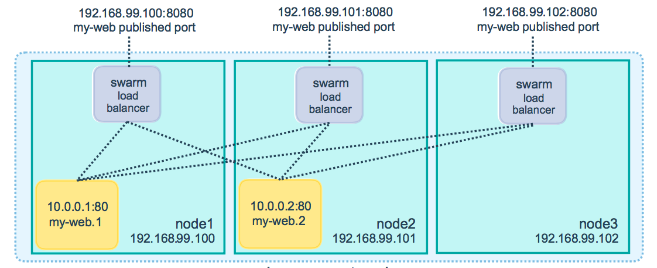
\includegraphics[width=10cm,height=4cm]{Images/C-2/swarmdiagramroute.png}
				\caption{Rute diagram ketika mode \textit{Swarm}\cite{docker_swarm_route}}
				\label{swarmdiagramroute}
			\end{figure}
		
			\indent Pada tugas akhir ini, \textit{Docker Swarm} akan digunakan sebagai manager atau okestrasi yang mengatur segala servis maupun aktivitas \textit{Docker Container} dan sebagai \textit{Load Balancer} untuk pembagian beban kontainer pada setiap \textit{nodes} yang merupakan instansi dari \textit{Docker Swarm} tersebut.
			
			
		
	\section{\textit{Laravel}}
		\textit{Laravel} adalah salah satu kerangka kerja yang berbahasa \textit{PHP} dan dibuat untuk memudahkan pengembang untuk mengembangan dan mendesain sebuah web yang menekankan kesederhanaan dan fleksibitas. Kerangka kerja ini mendukung metode \textit{MVC(Model-View-Controller)}. dimana \textit{MVC} digunakan untuk mengembangkan sebuah aplikasi yang memisahkan data(\textit{Model}) dari tampilan(\textit{View}) dan juga dari logika dari aplikasi tersebut(\textit{Controller})\cite{laraveframework}.
		
		\indent \textit{Model} digunakan untuk memanipulasi data dari basis data, \textit{View} berhubungan dengan antarmuka web seperti \textit{HTML}, \textit{CSS} dan \textit{JS} sebagai data pada pengguna. \textit{Controller} berhubungan dengan segala urusan logika pada servis web tersebut atau juga bisa disebut otaknya. \textit{Controller} juga berfungsi sebagai jembatan antara \textit{View} dan \textit{Model}\cite{laraveframework}.
	
		\indent Pada tugas akhir ini, kerangka kerja \textit{Laravel} akan digunakan untuk mengimplementasikan aplikasi web yang dibangun pada tugas akhir ini, dimana kerangka kerja ini sangat banyak digunakan oleh pengembang, memiliki dokumentasi resmi yang sangat baik, serta forum yang cukup baik. \textit{Laravel} yang akan digunakan adalah versi 5.8.
		
	\section{\textit{Python}}
		\textit{Python} adalah bahasa pemrograman tingkat tinggi yang didukung oleh struktur data \textit{built-in} semantik dinamis, selain itu Python mendukung pemrograman \textit{procedural}, \textit{object-oriented} dan \textit{functional}. \textit{Python} merupakan bahasa pemrograman \textit{interpreted}, oleh sebab itu, \textit{Python} tidak memakan biaya untuk kompilasi, sehingga proses pengembangan, pengujian dan \textit{debug} menjadi lebih cepat.
		 
		\indent Kelebihan bahasa pemrograman ini adalah memiliki modul dan \textit{package}, serta memiliki banyak standar pustaka yang didistribusikan secara bebas dan gratis. Selain itu \textit{Python} mudah dibaca karena memiliki sintaksis yang sederhana, sehingga dapat mengurangi biaya \textit{maintenance}. \textit{Debug} pada \textit{Python} juga mudah karena tidak akan terjadi \textit{segmentation fault}, namun akan memberi umpan balik berupa \textit{exception} apabila terdapat kesalahan atau \textit{error}\cite{python}.
		
		\indent Pada tugas akhir ini, Bahasa pemrograman \textit{Python} akan digunakan untuk mengimplementasikan algoritme \textit{task queue} pada sistem yang akan dibangun. \textit{Python} yang digunakan adalah versi 3.6.8.
	\chapter{DESAIN DAN PERANCANGAN}
    Pada bab ini dibahas mengenai analisis dan perancangan sistem.
    
    \section{Deskripsi Umum Sistem}
    	\indent Sistem yang akan dibangun pada tugas akhir ini adalah sebuah sistem yang dapat melakukan automasi uji beban terhadap suatu web. Uji beban pada sistem akan berjalan secara headless menggunakan sebuah tester yaitu Headless Chrome. Headless Chrome akan mendapatkan data uji beban ketika mengakses web yang diuji, sedangkan yang digunakan untuk mengambil data uji beban adalah sebuah pustaka Node yaitu Puppeteer. Sistem juga akan menggunakan Docker sebagai infrastruktur, sehingga Docker dapat digunakan sebagai load generator untuk melakukan uji beban yang bisa disebut kontainer.
    	
    	\indent Kontainer yang akan dipasang pada sistem membutuhkan sebuah alat orkestrasi untuk memanajemen kontainer secara otomatis, alat orkestrasi yang digunakan adalah Docker Swarm. Docker Swarm akan melibatkan 3 node host yang akan dibagi menjadi 1 node host sebagai swarm manager dan 2 node host sebagai worker. Docker Swarm akan bertanggung jawab dalam mendistribusikan kontainer ke masing-masing swarm node yang tergabung pada lingkungan swawrm atau bisa disebut sebagai load balancer.
    	
    	\indent Proses uji beban akan diproses user melakukan request skenario uji beban pada web service yang disediakan sistem. Kemudian controller pada web service akan mengirimkan skenario uji pada kontainer terpilih untuk melakukan pengujian. Setiap kontainer akan terinstall Headless Chrome dan Puppeteer. Headless Chrome akan mendapatkan data uji beban dan automasi pengambilan data uji beban dilakukan oleh Puppeteer. Puppeteer akan melakukan ekstraksi data uji beban menjadi satuan millisecond(ms). 
    	
    	\indent Sistem akan menyediakan basis data untuk menyimpan data yang diperlukan sistem. Basis data akan dipasang diluar lingkungan swarm dan lingkungan web service. Sistem juga menyediakan antarmuka pengguna berupa web yang akan digunakan untuk melihat laporan hasil uji beban. Sedangkan untuk mengatasi multiuser sistem akan menggunakan Task Scheduler atau Queue(antrian).
    
    \section{Kasus Penggunaan}
	    \begin{figure}[H]
	    	\centering
	    	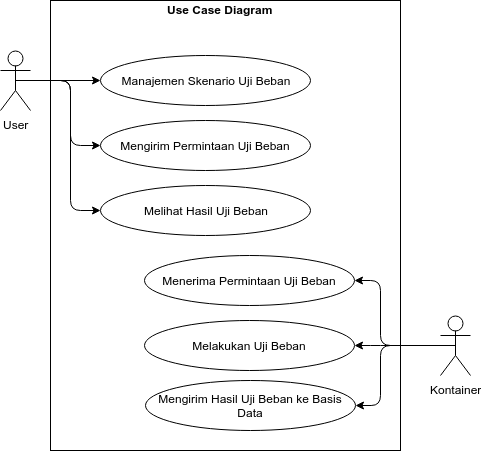
\includegraphics[width=9cm,height=9cm]{Images/C-3/usecasediagram.png}
	    	\caption{Diagram kasus penggunaan}
	    	\label{usecased}
	    \end{figure}
    	Terdapat dua aktor dalam sistem yang akan dibuat yaitu User dan Kontainer. User merupakan aktor yang bisa melakukan manajemen pada skenario yang ingin diuji dan melihat hasilnya, sedangkan Kontainer merupakan aktor yang akan digunakan sebagai load generator untu melakukan uji beban. Diagram kasus penggunaan digambarkan pada Gambar \ref{usecased} dan dijelaskan masing-masing pada Table \ref{tabelusecase}.
    	
    	\begin{longtable}{|p{0.20\textwidth}|p{0.30\textwidth}|p{0.35\textwidth}|}
    		\caption{Daftar kode kasus penggunaan} \label{tabelusecase} \\
    		\hline
    		\textbf{Kode Kasus Penggunaan} & \textbf{Nama Kasus Penggunaan} & \textbf{Keterangan} \\ \hline
    		\endhead
    		\endfoot
    		\endlastfoot
    		UC-0001 & Manajemen Skenario Uji Beban & User dapat menambah, melihat dan menghapus skenario uji beban \\ \hline
    		UC-0002 & Mengirim Permintaan Uji Beban & User dapat mengirimkan permintaan uji beban ke sistem melalui web service yang disediakan \\ \hline
    		UC-0003 & Melihat Hasil Uji Beban & Ketika proses uji beban selesai, user dapat melihat hasilnya di antarmuka pengguna web service yang disediakan \\ \hline
    		UC-0004 & Menerima Permintaan Uji Beban & Proses dimana kontainer akan menerima permintaan uji beban dari User \\ \hline
    		UC-0005 & Melakukan Uji Beban & Proses dimana kontainer akan melakukan uji beban sesuai skenario yang dikirim \\ \hline
    		UC-0006 & Mengirim Hasil Uji Beban ke Basis Data & Ketika kontainer telah selesai melakukan pengujian, data yang didapatkan akan dikirim ke basis data MySQL \\ \hline
    	\end{longtable}
    
    \section{Arsitektur Sistem}
	    \begin{figure}[H]
	    	\centering
	    	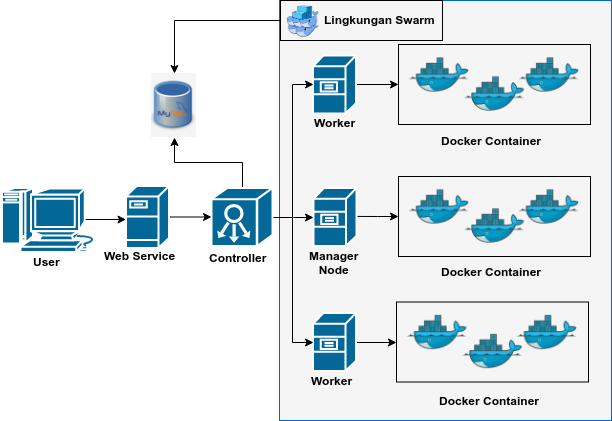
\includegraphics[width=10cm,height=6cm]{Images/C-3/arsitektursistem.png}
	    	\caption{Desain arsitektur sistem}
	    	\label{arsitekturumum}
	    \end{figure}
    	
    	\indent Pada sub-bab ini, akan dibahas mengenai tahap analisis arsitektur, analisis teknologi dan desain sistem yang akan dibangun. Arsitektur sistem secara umum ditunjukkan pada Gambar \ref{arsitekturumum}.

    	\subsection{Desain Umum Sistem}
    		Berdasarkan yang dijelaskan pada deskripsi umum sistem, dapat diperoleh beberapa kebutuhan sistem antara lain:
    		\begin{enumerate}
    			\item Load generator untuk melakukan uji beban.
    			\item Tester yang bisa mengambil data uji beban.
    			\item Web service sebagai antarmuka pengguna.
    			\item Basis data untuk menyimpan data sistem.
    			\item Task Queue untuk menangani kasus request lebih dari satu user.
    		\end{enumerate}
    	
    		Untuk memenuhi kebutuhan sistem yang dijelaskan sebelumnya, penulis membagi menjadi beberapa komponen sistem yang akan digunakan pada tugas akhir ini.
    		
    		\begin{enumerate}
    			\item Load generator \\
    				Berfungsi sebagai pengganti user yang akan melakukan akses web melalui browser.
    			\item Pengambil data uji beban \\
    				Berfungsi untuk mengambil data uji beban ketika load generator mengakses web dari browser.
    			\item Service Controller \\
    				Berfungsi sebagai pengatur sistem uji beban yang terdiri :
    				\begin{itemize}
    					\item Web Service \\
    						Berfungsi sebagai tampilan antarmuka pengguna untuk menggunakan sistem.
    					\item Basis Data \\
    						Berfungsi untuk menyimpan data yang digunakan untuk menyimpan segala data yang dibutuhkan oleh sistem.
    					\item Task Queue \\
    						Berfungsi untuk membuat task scheduler atau antrian untuk menangani kasus request lebih dari satu user.
    				\end{itemize}
    		\end{enumerate}
    	
    	\subsection{Perancangan Load Generator}
	    	\begin{figure}[h]
	    		\centering
	    		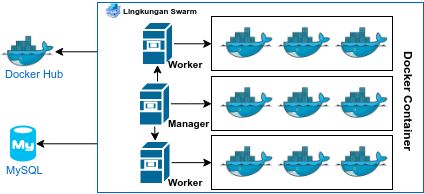
\includegraphics[width=11cm,height=6cm]{Images/C-3/dockerdesain.png}
	    		\caption{Desain perancangan load generator}
	    		\label{dockerdesain}
	    	\end{figure}
    		Komponen load generator akan difungsikan sebagai pengganti pengguna yang mengakses ke suatu web melalui browser. Komponen yang akan digunakan sebagai load generator adalah Docker atau bisa disebut kontainer. Ketika melakukan pemasangan kontainer sebuah Docker Image, untuk memenuhi hal tersebut, pada tugas akhir ini penulis akan membuat sebuah Docker Image yang akan diunggah ke Docker Hub. Sehingga ketika akan memasang kontainer pada node host yang baru, node host tersebut hanya perlu mengunduh Docker Image yang telah diunggah sebelumnya. Seluruh kontainer akan dibangun di dalam lingkungan swarm untuk memudahkan dalam mengatur atau memanajemen kontainer ke semua node host yang tergabung di dalam lingkungan swarm, sedangkan untuk memudahkan akses ke setiap kontainer, maka data dari kontainer akan disimpan di dalam basis data MySQL. Load generator akan terdiri dari 3 node host, 1 sebagai manager node dan 2 lainnya sebagai worker, sedangkan basis data akan berada di luar lingkungan swarm. Desain perancangan komponen ini digambarkan pada Gambar \ref{dockerdesain}.
    		 
    	
    	\subsection{Perancangan Pengambil Data Uji Beban}
    		Komponen ini akan membutuhkan suatu alat yang bisa mendapatkan data uji beban terlebih dahulu. Pada tugas akhir ini, akan menggunakan Headless Chrome untuk mendapatkan data uji beban ketika mengakses web. Setelah mendapatkan data uji beban, diperlukan juga suatu alat yang bisa digunakan untuk mengambil data uji beban pada Headless Chrome, alat tersebut adalah Puppeteer. Puppeteer akan melakukan pengambilan secara otomatis ketika ada perintah yang masuk dan menyimpan data uji beban pada basis data MySQL. Alat-alat yang digunakan pada komponen ini akan dipasang pada masing-masing kontainer di setiap node host. Desain perancangan komponen ini digambarkan pada Gambar \ref{puppdesain}.
    		\begin{figure}[H]
    			\centering
    			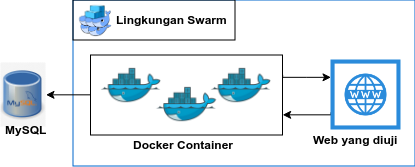
\includegraphics[width=10cm,height=4.5cm]{Images/C-3/puppdesain.png}
    			\caption{Desain pengambil data uji beban}
    			\label{puppdesain}
    		\end{figure}
    	
    	\subsection{Perancangan Service Controller}
    		Komponen ini akan digunakan untuk mengatur segala proses uji beban pada sistem. Pada komponen ini akan terdapat 3 buah sub-komponen yaitu web service, basis data dan task queue atau antrian.
    	
	    	\subsubsection{Desain Web Service}
	    		Web service akan berfungsi sebagai antarmuka pengguna dan sebagai penghubung antara user dengan kontainer. Antarmuka pengguna berfungsi memudahkan user untuk membuat skenario yang akan dikirimkan ke load generator dan kemudian load generator akan melakukan uji beban sesuai dengan skenario yang dikirim user melalui web service. Sedangkan untuk mengatur segala aktivitas user dibutuhkan sebuah controller dan rute yang akan dipasang pada web service. Desain antarmuka pengguna ditunjukkan pada Gambar \ref{mockupweb}.
	    		\begin{figure}[H]
	    			\centering
	    			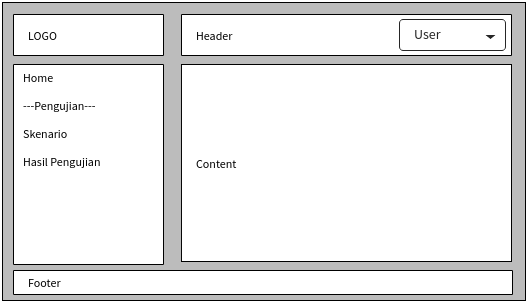
\includegraphics[width=10cm,height=6cm]{Images/C-3/mockupweb.png}
	    			\caption{Desain antarmuka pengguna}
	    			\label{mockupweb}
	    		\end{figure}
	    	
		    	Selain itu, akan dirancang juga fitur-fitur pada web service yang akan digunakan user antara lain:
		    	\begin{enumerate}
		    		\item Menambah dan menghapus skenario.
		    		\item Menentukan jumlah worker pengujian.
		    		\item Melihat performa hasil pengujian.
		    		\item Melihat tangkapan layar tampilan web yang diuji.
		    		\item Melihat console error.
		    		\item Melihat status antrian proses uji. \\
		    	\end{enumerate}
	    		
	   		\subsubsection{Desain Basis Data}
	   			Komponen basis data diperlukan untuk menyimpan data-data yang berkaitan dengan sistem. data yang disimpan adalah data node host swarm, data kontainer, data pengguna, data skenario pengujian, data antrian request, data hasil pengujian, data error console, data rata-rata hasil pengujian. Dari data-data tersebut maka dibutuhkan suatu tabel diantaranya yaitu:
	   			\begin{itemize}
	   				\item Tabel swarms \\
	   					Menyimpan data nohe host yang tergabung di dalam lingkungan swarm.
	   				\item Tabel containers \\
	   					Menyimpan data Docker Container yang telah dipersiapkan.
	   				\item Tabel users \\
	   					Menyimpan data pengguna.
	   				\item Tabel scenarios \\
	   					Menyimpan data skenario pengujian.
	   				\item Tabel queues \\
		   				Menyimpan data antrian request pengujian dari user.
	   				\item Tabel results \\
	   					Menyimpan data hasil pengujian yang dilakukan setiap kontainer.
	   				\item Tabel errors \\
	   					Menyimpan data console error yang ada di browser.
	   				\item Tabel summary results \\
	   					Menyimpan data rata-rata hasil pengujian setiap skenario.
	   			\end{itemize}
	    		
	    	\subsubsection{Desain Penggunaan Task Queue}
	    		Pada service controller akan ada banyak request dari user, setiap request tentu saja akan terdapat proses yang akan berjalan dalam jangka waktu yang cukup lama. Jika proses tersebut berada di dalam fungsi yang dipanggil melalui protokol HTTP, maka akan memberikan umpan balik setelah semua proses yang ada dibaliknya selesai. Hal ini akan membuat user yang melakukan request perlu menunggu dan tidak efisien. Untuk mengatasi hal ini, akan dirancang sebuah komponen antrian atau bisa disebut task queue. Task queue akan membuat antrian untuk setiap request dibelakang layar. Antrian request tersebut akan disimpan pada basis data MySQL.
	\chapter{IMPLEMENTASI}
	Bab ini membahas mengenai implementasi dari sistem yang sudah di desain dan dirancang pada bab sebelumnya. Pembahasan secara rinci akan dijelaskan pada setiap komponen yang ada yaitu \textit{load generator}, pengambil data uji beban dan \textit{service controller} yang meliputi \textit{web service}, basis data dan \textit{task queue}.
	
	\section{Lingkungan Implementasi}
		Dalam mengimplementasikan sistem pada tugas akhir ini, digunakan beberapa perangkat pendukung sebagai berikut.
		
		\subsection{Perangkat Keras}
		Perangkat keras yang digunakan dalam pengembangan sistem adalah sebagai berikut:
		\begin{enumerate}
			\item \textit{Web service} dan \textit{task queue}, \textit{processor} AMD FX-7600P Radeon R7, 12 Compute Cores 4C+8G dan RAM 8GB.
			\item \textit{Node swarm} dengan IP 167.71.194.235, \textit{processor} Intel(R) Xeon(R) CPU E5-2650 v4@2.20GHz dan RAM 4GB.
			\item \textit{Node swarm} dengan IP 165.22.55.82, \textit{processor} Intel(R) Xeon(R) CPU E5-2650 v4@2.20GHz dan RAM 4GB.
			\item \textit{Node swarm} dengan IP 167.71.194.233, \textit{processor} Intel(R) Xeon(R) CPU E5-2650 v4@2.20GHz dan RAM 4GB.
			\item Basis data \textit{MySQL} dengan IP 178.128.123.143, \textit{processor} Intel(R) Xeon(R) Gold 6140 CPU@2.30GHz dan RAM 1GB.
		\end{enumerate}
	
		\subsection{Perangkat Lunak}
		Perangkat lunak yang digunakan dalam pengembangan sistem adalah sebagai berikut:
		\begin{enumerate}
			\item Sistem Operasi \textit{Ubuntu} 18.04 LTS 64 Bit
			\item \textit{Docker} versi 18.09.6 
			\item \textit{Headless Chrome} 
			\item \textit{Puppeteer} versi 0.12.0
			\item \textit{NPM} versi 6.4.1
			\item \textit{Node.js} versi 8.15.1
			\item \textit{Python} versi 3.6.8
			\item \textit{MySQL} Ver 14.14 Distrib 5.7.26
			\item \textit{Shell Script}
			\item \textit{PHP} dan \textit{Laravel} versi 5.8
		\end{enumerate}
		
	\section{Implementasi \textit{Load Generator}}
		Berdasarkan perancangan dan desain, \textit{load generator} merupakan aktor yang akan berfungsi menggantikan pengguna ketika mengakses ke web. \textit{Load generator} yang akan digunakan adalah \textit{Docker}, namun diperlukan beberapa tahap untuk bisa menggunakan \textit{Docker} atau kontainer sebagai \textit{load generator}, yaitu tahap pemasangan dan konfigurasi. Tahap pemasangan \textit{Docker} dapat dilihat di Kode Sumber \ref{instalasidocker}, sedangkan untuk konfigurasi akan dibagi menjadi beberapa tahap yaitu:
		\begin{enumerate}
			\item Pembuatan \textit{Docker Image}
			\item Pembuatan lingkungan kontainer
			\item Pemasangan \textit{Headless Chrome} dan \textit{Puppeteer}
		\end{enumerate}
			
		\subsection{Implementasi Pembuatan \textit{Docker Image}}
			\textit{Docker Image} digunakan untuk menjalankan kontainer, pada tugas akhir ini \textit{Docker Image} akan dibuat terlebih dahulu agar bisa digunakan untuk menjalankan \textit{Puppeteer} dan \textit{Headless Chrome}. Namun untuk membuat \textit{Docker Image} diperlukan beberapa tahapan yaitu konfigurasi \texttt{Dockerfile}, pemasangan \textit{Docker Compose} dapat dilihat pada Kode Sumber \ref{dockercomposeinstall} dan konfigurasi \texttt{docker-compsoe.yml} dan unggah \textit{Docker Image} ke \textit{Docker Hub}.
			
			\indent Konfigurasi \texttt{Dockerfile} dapat dilihat pada Kode Sumber \ref{dockerimage}, sedangkan konfigurasi \texttt{docker-compose.yml} dapat dilihat pada Kode Sumber \ref{dockercompose}.
				\begin{lstlisting}[frame=single,tabsize=2,breaklines,caption={Konfigurasi \textit{Dockerfile} },label=dockerimage, captionpos=b, language=json]
	FROM node:8
	RUN apt-get update
	# for https
	RUN apt-get install -yyq ca-certificates
	# install libraries
	RUN apt-get install -yyq libappindicator1 libasound2 libatk1.0-0 libc6 libcairo2 libcups2 libdbus-1-3 libexpat1 libfontconfig1 libgcc1 libgconf-2-4 libgdk-pixbuf2.0-0 libglib2.0-0 libgtk-3-0 libnspr4 libnss3 libpango-1.0-0 libpangocairo-1.0-0 libstdc++6 libx11-6 libx11-xcb1 libxcb1 libxcomposite1 libxcursor1 libxdamage1 libxext6 libxfixes3 libxi6 libxrandr2 libxrender1 libxss1 libxtst6
	# tools
	RUN apt-get install -yyq gconf-service lsb-release wget xdg-utils
	RUN apt-get install -yyq fonts-liberation 
	COPY code /app/code
	COPY output /app/output
	WORKDIR /app/code
	RUN yarn install
				\end{lstlisting}
				
				\begin{lstlisting}[frame=single,tabsize=2,breaklines,caption={Konfigurasi \textit{docker-compose.yml} },label=dockercompose, captionpos=b, language=json]
	version: '3'
	services:
		puppeteer:
			build: .
			shm_size: '1gb'
			entrypoint: ["sh", "-c", "sleep infinity"]
				\end{lstlisting}
				
				Kemudian jalankan perintah \textit{Docker Compose} berikut untuk pembuatan \textit{Docker Image}.
				\begin{lstlisting}[frame=single,tabsize=2,breaklines,caption={Perintah untuk menjalankan  \textit{Docker Compose}},label=createimg, captionpos=b, language=json,numbers=none]
	$ docker-compose up
				\end{lstlisting}
				
				Setelah \textit{Docker Image} terbuat, ubah nama \textit{Docker Image} tersebut dan melakukan \textit{commit} agar bisa di \textit{push}. Perintah pada kode sumber \ref{pushimagedocker} yang digunakan oleh penulis ketika mengunggah \textit{Docker Image} ke \textit{Docker Hub}.
				\begin{lstlisting}[frame=single,tabsize=2,breaklines,caption={Perintah untuk mengunggah \textit{Docker Image}},label=pushimagedocker, captionpos=b, language=json,numbers=none]
	$ docker tag puppeteer_puppeteer:latest cphikmawan/ta2019:newpupp
	
	$ docker push cphikmawan/ta2019:newpupp
				\end{lstlisting}
				
		\subsection{Implementasi Pembuatan Lingkungan Kontainer}
			Kontainer akan dipasangkan pada suatu lingkungan yang bisa mengatur segala aktivitas kontainer, lingkungan yang akan dibangun pada sistem menggunakan alat orkestrasi yaitu \textit{Docker Swarm}. Untuk mengimplementasikan \textit{Docker Swarm} pada sistem ini, dibutuhkan satu \textit{node host} sebagai \textit{manager node} dan dua lainnya sebagai \textit{worker}. Tahap pertama yang dilakukan yaitu menginisiasi salah satu \textit{node host} yang akan digunakan sebagai \textit{manager node}. Perintah inisiasi \textit{manager node} terdapat pada Kode Sumber \ref{swarminit}.
			\begin{lstlisting}[frame=single,tabsize=2,breaklines,caption={Perintah untuk inisiasi \textit{manager node}},label=swarminit, captionpos=b, language=json,numbers=none]
	$ docker swarm init --advertise-addr [IP NODE]
			\end{lstlisting}
			
			Setelah perintah pada kode sumber \ref{swarminit} dijalankan, maka \textit{manager node} akan menghasilkan sebuah token yang digunakan oleh \textit{node host} yang lain untuk bergabung sebagai \textit{worker}. Perintah yang harus dijalankan pada setiap \textit{node host} yang lain terdapat pada Kode Sumber \ref{swarmjoin}.
			\begin{lstlisting}[frame=single,tabsize=2,breaklines,caption={Perintah untuk bergabung ke \textit{Swarm}},label=swarmjoin, captionpos=b, language=json,numbers=none]
	$ docker swarm join --token [token] [IP MANAGER]:2377
			\end{lstlisting}
			
			Tahap terakhir yang dilakukan yaitu memastikan semua \textit{node host} sudah tergabung dengan \textit{manager node}.
			\begin{lstlisting}[frame=single,tabsize=2,breaklines,caption={Perintah untuk melihat daftar \textit{Swarm Node}},label=dockernodels, captionpos=b, language=json,numbers=none]
	$ docker node ls
			\end{lstlisting}
			
		\subsection{Implementasi Pemasangan \textit{Headless Chrome} dan \textit{Puppeteer}}
			\textit{Headless Chrome} dan \textit{Puppeteer} akan dipasang pada masing-masing kontainer menggunakan \textit{Docker Image} yang telah dibuat sebelumnya, untuk pemasangannya akan dilakukan dilingkungan \textit{Docker Swarm} dan dilakukan pada \textit{manager node}. Namun untuk implementasinya dibutuhkan beberapa persiapan dan konfigurasi yang harus dilakukan terlebih dahulu yaitu konfigurasi unduh \textit{Docker Image}, konfigurasi membuat \textit{Docker Network}, konfigurasi \textit{puppeteer.yml}, konfigurasi \textit{deployment}.
			
			\indent Untuk mengunduh \textit{Docker Image} dilakukan pada setiap \textit{node host} menggunakan perintah pada Kode Sumber \ref{unduhimage} dan membuat \textit{Docker Network} pada Kode Sumber \ref{createnetwork}. Sedangkan konfigurasi \texttt{puppeteer.yml} dapat dilihat di Kode Sumber \ref{puppyaml}
			\begin{lstlisting}[frame=single,tabsize=2,breaklines,caption={Perintah untuk mengunduh \textit{Docker Image} },label=unduhimage, captionpos=b, language=json,numbers=none]
	$ docker image pull cphikmawan/ta2019:puppeteer
			\end{lstlisting}
			
			\begin{lstlisting}[frame=single,tabsize=2,breaklines,caption={Perintah untuk membuat\textit{ Docker Network} },label=createnetwork, captionpos=b, language=json,numbers=none]
	$ docker network create \
		--driver overlay \
		--subnet 10.0.0.0/18 \
		--attachable \
		[nama_network]
			\end{lstlisting}
			
			\begin{lstlisting}[frame=single,tabsize=2,breaklines,caption={Konfigurasi \textit{puppeteer.yml}},label=puppyaml, captionpos=b, language=json]
	version: '3'
	# konfigurasi service
	services:
		# nama service yang akan dibuat
		puppeteer:
			# docker image yang digunakan
			image: cphikmawan/ta2019:newpupp
			# sinkronisasi penyimpanan antara kontainer dengan host
			volumes:
				- ./output:/app/output
				- ./code:/app/code
			# direktori kerja didalam kontainer
			working_dir: /app/code
			# konfigurasi untuk jumlah kontainer dan handling
			deploy:
				replicas: 1000
				restart_policy:
					condition: on-failure
			# entrypoint awal tidak akan melakukan apapun
			entrypoint: ["sh", "-c", "sleep infinity"]
	# konfigurasi jaringan
	networks:
		default:
			# jaringan default akan diubah ke jaringan eksternal
			external:
				# akan terkonek ke jaringan "swarm-network"
				name: swarm-network
			\end{lstlisting}
			
			\indent Tahap selanjutnya adalah konfigurasi \textit{deployment} dengan menjalankan perintah yang ditunjukkan pada Kode Sumber \ref{pemasanganstack} di terminal \textit{manager node}
			\begin{lstlisting}[frame=single,tabsize=2,breaklines,caption={Perintah untuk pemasangan kontainer },label=pemasanganstack, captionpos=b, language=json,numbers=none]
	$ docker stack deploy --compose-file=puppeteer.yml [nama_stack]
			\end{lstlisting}
	
	\section{Implementasi Pengambil Data Uji Beban}
		Pengambil Data Uji Beban akan dilakukan menggunakan sebuah pustaka \textit{Node} yaitu \textit{Puppeteer}. Pada saat dilakukan uji beban, \textit{Puppeteer} akan mengambil data uji beban dari \textit{Headless Chrome} menggunakan \textit{API} dari \textit{Puppeteer} secara otomatis. Beberapa data uji beban yang akan diambil yaitu:
		\begin{enumerate}
			\item \textit{Response End} \\
				Atribut ini menunjukkan waktu setelah \textit{user} menerima \textit{byte} terakhir dari dokumen sebelum koneksi transportasi ditutup.
			\item \textit{DOM Content Loaded} \\
				Atribut ini menunjukkan waktu setelah dokumen sudah diterima oleh \textit{user}.
			\item \textit{Load Event End} \\
				Atribut ini mengembalikan waktu ketika memuat dokumen selesai.
			\item \textit{CSS Tracing End} \\
				Atribut ini menunjukkan waktu dari ekstraksi akhir file \textit{CSS} dimuat.
			\item \textit{First Meaningfulpain} \\
				Atribut ini adalah atribut khusus yang ada pada \textit{Chrome} yang menunjukkan bahwa segala konten halaman yang dimuat sudah ditampilkan di layar. \\
		\end{enumerate}
	 
	 	\indent Selain data uji beban diatas, \textit{Puppeteer} juga digunakan untuk mengambil sebuah tangkapan layar sesuai skenario yang dikirimkan oleh pengguna dan mengambil data saat terjadi kegagalan saat memuat \textit{assets} yang tertulis pada \textit{console browser}. Adapun \textit{pseudocode} untuk melakukan pengambilan data uji beban dapat dilihat pada Kode Sumber \ref{pseudocodepupp}.
	 	
	 	\begin{lstlisting}[frame=single,tabsize=2,breaklines,caption={\textit{Pseudocode Puppeteer}},label=pseudocodepupp, captionpos=b, language=json]
 	Variable Declaration
 	Data = Read Scenario File Configuration
 	
 	TESTPAGE FUNCTION:
 		CALL HELPERS FUNCTION:
 			GET Navigation Start
 		START Trace CSS Data
 		Trying to Accessing Website
 		END Trace CSS Data
 		CALL HELPERS FUNCTION:
 			GET Extracted Performance Data
 			GET Extracted CSS Tracing
 			RETURN Extracted Data
 	END TESTPAGE FUNCTION
 	
 	HELPERS FUNCTION:
 		GET Navigation Start
 			RETURN Navigation Start
 		Extracted Performance Data = Performance Data * 1000 - Navigation Start
 			RETURN Extracted Performance Data
 		Extracted CSS Tracing = CSS Tracing / 1000
 			RETURN Extracted CSS Tracing 
 	End Helpers Function
 	
 	MAIN FUNCTION:
 		START Headless Browser
 		GET Error Console
 			RETURN Data to Database
 		TRY:
 			CALL TESTPAGE FUNCTION(Data):
 				Get Data From TestPage -> Save Data Uji Beban
 			GET Page Screenshoot -> Save Screenshoot
 		CATCH ERROR:
 			GET Error
 			GET Page Screenshoot -> Save Screenshoot
 	END MAIN FUNCTION
	 	\end{lstlisting}
	
	\section{Implementasi \textit{Service Controller}}
		Berdasarkan desain dan perancangan, \textit{service controller} terdiri dari komponen \textit{web service}, basis data dan \textit{task queue}. Komponen tersebut akan diimplementasikan pada satu komputer milik penulis yang akan digunakan untuk \textit{web service} dan penggunaan \textit{task queue}, serta satu buah server untuk basis data \textit{MySQL}.
		
		\subsection{Implementasi \textit{Web Service}}
			Pada implementasi \textit{web service} dibutuhkan beberapa persiapan lingkungan yang perlu dilakukan, urutannya meliputi langkah-langkah berikut:
			\begin{enumerate}
				\item Instalasi \textit{PHP}
				\item Instalasi \textit{Composer}
				\item Instalasi \textit{Laravel} versi 5.8
				\item Instalasi \textit{MySQL}
			\end{enumerate}
			
			\indent \textit{Web service} akan menggunakan bahasa \textit{PHP} dan kerangka kerja \textit{Laravel} versi 5.8, sedangkan \textit{Composer} berfungsi untuk memanajemen instalasi pustaka pada \textit{PHP} dan untuk penyimpanan data yang digunakan pada sistem akan disimpan pada basis data \textit{MySQL}. \textit{Web service} berfungsi untuk memudahkan pengguna melakukan uji beban pada suatu web. Tampilan antarmuka pengguna ditunjukkan pada Gambar \ref{gambarweb}.
			
			\begin{figure}[H]
				\centering
				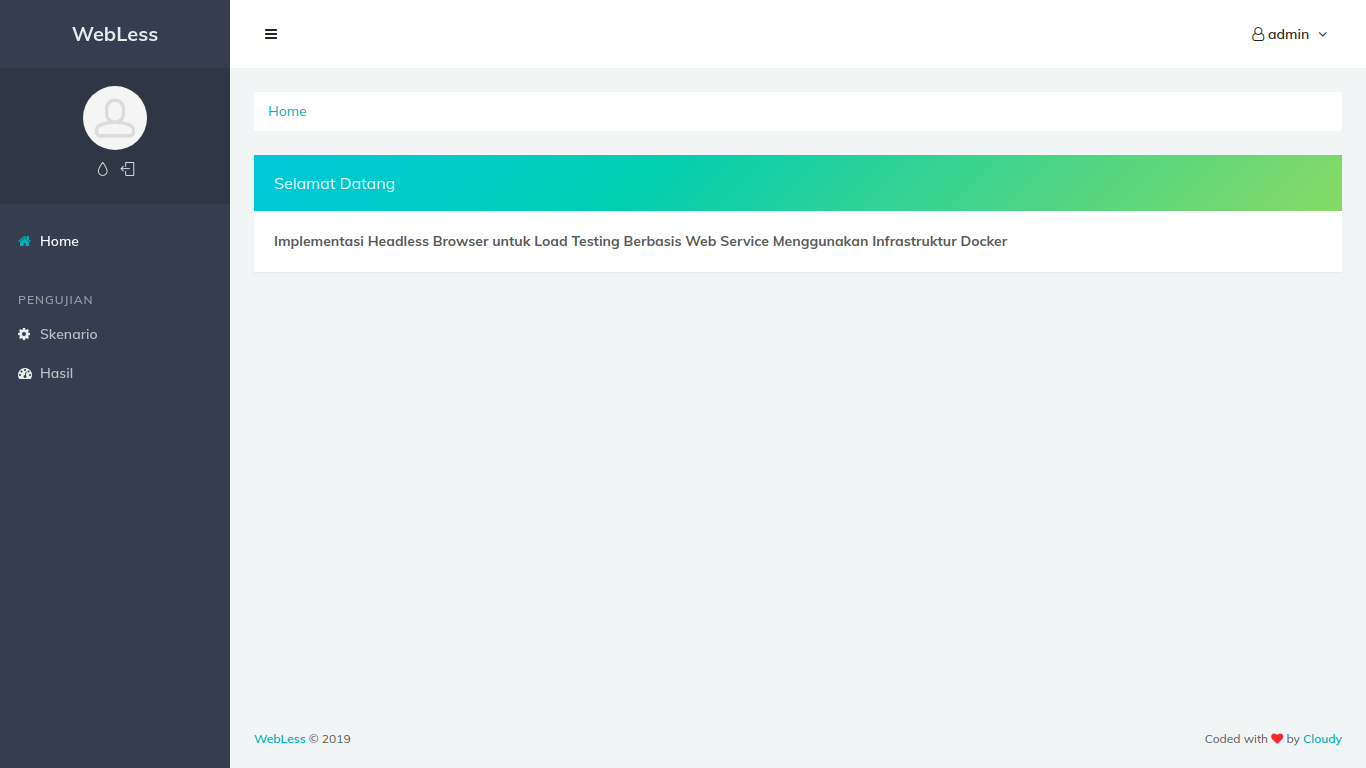
\includegraphics[width=10cm,height=6cm]{Images/C-4/gambarweb.png}
				\caption{Tampilan web antarmuka pengguna}
				\label{gambarweb}
			\end{figure}
			
			\indent \textit{Web service} memiliki beberapa rute \textit{HTTP} yang akan digunakan oleh pengguna ketika mengakses web sistem. Rute-rute tersebut ditunjukkan pada Tabel \ref{tabelruteweb}.
			\begin{longtable}{|p{0.05\textwidth}|p{0.25\textwidth}|p{0.30\textwidth}|p{0.30\textwidth}|}
				\caption{Rute \textit{HTTP} pada \textit{web service}} \label{tabelruteweb} \\ \hline
				\textbf{No} & \textbf{Rute} & \textbf{Metode} & \textbf{Aksi} \\ \hline
				\endhead
				\endfoot
				\endlastfoot
				1 & / & GET & Mengakses halaman \textit{home} \\ \hline
				2 & /login & GET & Mengakses halaman \textit{login} \\ \hline
				3 & /login & POST & Melakukan \textit{login} \\ \hline
				4 & /logout & GET & Melakukan \textit{logout} \\ \hline
				5 & /skenario & GET & Melihat skenario \\ \hline
				6 & /skenario/create & GET & Mengakses halaman tambah skenario \\ \hline
				7 & /skenario & POST & Menambahkan skenario \\ \hline
				8 & /skenario/{id} & DELETE & Menghapus skenario \\ \hline
				9 & /worker & GET & Mengakses halaman \textit{worker} \\ \hline
				10 & /worker & POST & Menambahkan jumlah \textit{worker(load generator)} dan data antrian \\ \hline
				11 & /hasil/rata-rata & GET & Mendapatkan hasil pengujian \\ \hline
				12 & /hasil/error-console & GET & Mendapatkan \textit{error console} web \\ \hline
				13 & /hasil/images & GET & Melihat tangkapan layar web \\ \hline
				14 & /antrian & GET & Melihat jumlah dan status antrian \\ \hline
				
			\end{longtable}
		
		\subsection{Implementasi Skema Basis Data}
			Berdasarkan hasil perancangan basis data pada bab sebelumnya. Data yang dibutuhkan dan digunakan oleh sistem akan disimpan di dalam basis data \textit{MySQL}. Data yang disimpan adalah data \textit{node host swarm}, data kontainer, data pengguna, data skenario pengujian, data antrian \textit{request}, data hasil pengujian, data \textit{error console}, data rata-rata hasil pengujian.
			
			\subsubsection{Tabel \textit{Swarms}}
				Pada tabel \textit{swarms} menyimpan data-data dari node host yang tergabung dilingkungan \textit{swarm}. Berikut definisi tabel \textit{swarms} pada Tabel \ref{tabelswarms}.
				
				\begin{longtable}{|p{0.05\textwidth}|p{0.30\textwidth}|p{0.20\textwidth}|p{0.35\textwidth}|}
					\caption{Tabel \textit{swarms}} \label{tabelswarms} \\
					\hline
					\textbf{No} & \textbf{Kolom} & \textbf{Tipe} & \textbf{Keterangan} \\ \hline
					\endhead
					\endfoot
					\endlastfoot
					1 & id & bigint(20) & Sebagai \textit{primary key}, nilai awal adalah \textit{auto\_increment}. \\ \hline
					2 & swarm\_ip & varchar(255) & Menunjukkan \textit{IP} dari \textit{node host} \\ \hline
					3 & swarm\_username & varchar(255) & Menunjukkan \textit{username} dari \textit{node host} \\ \hline
					4 & swarm\_password & varchar(255) & Menunjukkan \textit{password} dari \textit{node host} \\ \hline
					5 & is\_used & smallint(6) & Menunjukkan status dari \textit{node host} \\ \hline
				\end{longtable}
		
			\subsubsection{Tabel \textit{Containers}}
				Padata tabel \textit{containers} menyimpan data-data dari \textit{Docker Container} yang akan digunakan sebagai \textit{load generator}. Berikut definisi tabel \textit{containers} pada Tabel \ref{tabelcontainers}.
				
				\begin{longtable}{|p{0.05\textwidth}|p{0.30\textwidth}|p{0.20\textwidth}|p{0.35\textwidth}|}
					\caption{Tabel \textit{containers}} \label{tabelcontainers} \\
					\hline
					\textbf{No} & \textbf{Kolom} & \textbf{Tipe} & \textbf{Keterangan} \\ \hline
					\endhead
					\endfoot
					\endlastfoot
					1 & id & bigint(20) & Sebagai \textit{primary key}, nilai awal adalah \textit{auto\_increment} \\ \hline
					2 & task\_id & varchar(100) & Menunjukkan \textit{task id} dari kontainer \\ \hline
					3 & node\_id & varchar(100) & Menunjukkan \textit{node id} tempat kontainer dipasang \\ \hline
					4 & container\_id & varchar(100) & Menunjukkan \textit{id} dari kontainer \\ \hline
					5 & node\_ip & varchar(100) & Menunjukkan \textit{IP} tempat kontainer dipasang \\ \hline
					6 & node\_host & varchar(100) & Menunjukkan \textit{hostname} tempat kontainer dipasang \\ \hline
					7 & status & smallint(6) & Menunjukkan \textit{flag} status dari \textit{container} \\ \hline
					8 & username & varchar(100) & Menunjukkan status kontainer yang sedang digunakan \textit{user} \\ \hline
				\end{longtable}
		
			\subsubsection{Tabel \textit{Users}}
				Pada tabel \textit{users} menyimpan data-data pengguna web yang disediakan sistem. Berikut definisi tabel \textit{users} pada Tabel \ref{tabelusers}. Data pengguna juga memiliki \textit{constraint} dan disimpan pada Tabel \textit{role\_user} \ref{tabelroleuser} dan Tabel \textit{roles} \ref{tabelroles}.
				
				\begin{longtable}{|p{0.05\textwidth}|p{0.30\textwidth}|p{0.20\textwidth}|p{0.35\textwidth}|}
					\caption{Tabel \textit{users}} \label{tabelusers} \\
					\hline
					\textbf{No} & \textbf{Kolom} & \textbf{Tipe} & \textbf{Keterangan} \\ \hline
					\endhead
					\endfoot
					\endlastfoot
					1 & id & bigint(20) & Sebagai \textit{primary key}, nilai awal adalah \textit{auto\_increment} \\ \hline
					2 & name & varchar(255) & Menunjukkan nama pengguna \\ \hline
					3 & email & varchar(255) & Menunjukkan \textit{email} pengguna \\ \hline
					4 & username & varchar(255) & Menunjukkan \textit{username} pengguna \\ \hline
					5 & password & varchar(255) & Menunjukkan \textit{password} pengguna \\ \hline
				\end{longtable}
			
				\begin{longtable}{|p{0.05\textwidth}|p{0.30\textwidth}|p{0.20\textwidth}|p{0.35\textwidth}|}
					\caption{Tabel \textit{role\_user}} \label{tabelroleuser} \\
					\hline
					\textbf{No} & \textbf{Kolom} & \textbf{Tipe} & \textbf{Keterangan} \\ \hline
					\endhead
					\endfoot
					\endlastfoot
					1 & id & bigint(20) & Sebagai \textit{primary key}, nilai awal adalah \textit{auto\_increment} \\ \hline
					2 & role\_id & int(10) & Menunjukkan \textit{id role} pengguna \\ \hline
					3 & user\_id & int(10) & Menunjukkan \textit{id} pengguna \\ \hline
				\end{longtable}
				
				\begin{longtable}{|p{0.05\textwidth}|p{0.30\textwidth}|p{0.20\textwidth}|p{0.35\textwidth}|}
					\caption{Tabel \textit{roles}} \label{tabelroles} \\
					\hline
					\textbf{No} & \textbf{Kolom} & \textbf{Tipe} & \textbf{Keterangan} \\ \hline
					\endhead
					\endfoot
					\endlastfoot
					1 & id & bigint(20) & Sebagai \textit{primary key}, nilai awal adalah \textit{auto\_increment} \\ \hline
					2 & name & varchar(255) & Menunjukkan nama \textit{role} \\ \hline
					3 & description & varchar(255) & Menunjukkan deskripsi hak akses dari nama \textit{role} \\ \hline
				\end{longtable}
		
			\subsubsection{Tabel \textit{Scenarios}}
				Pada tabel \textit{scenarios} menyimpan data-data skenario yang telah dibuat oleh pengguna. Berikut definisi tabel \textit{scenarios} pada Tabel \ref{tabelscenarios}.
			
				\begin{longtable}{|p{0.05\textwidth}|p{0.30\textwidth}|p{0.20\textwidth}|p{0.35\textwidth}|}
					\caption{Tabel scenarios} \label{tabelscenarios} \\
					\hline
					\textbf{No} & \textbf{Kolom} & \textbf{Tipe} & \textbf{Keterangan} \\ \hline
					\endhead
					\endfoot
					\endlastfoot
					1 & id & bigint(20) & Sebagai \textit{primary key}, nilai awal adalah \textit{auto\_increment} \\ \hline
					2 & scenario\_id & varchar(255) & Menunjukkan skenario \textit{id} sebagai \textit{foreign key} \\ \hline
					3 & username & varchar(255) & Menunjukkan keterangan pengguna pembuat skenario \\ \hline
					4 & scenario\_method & varchar(255) & Menunjukkan metode uji \\ \hline
					5 & scenario\_link & varchar(255) & Menunjukkan \textit{link} \textit{website} yang diuji \\ \hline
					6 & scenario\_worker & varchar(255) & Menunjukkan jumlah \textit{load generator} yang diinginkan pengguna \\ \hline
					7 & scenario\_status & smallint(6) & Menunjukkan status skenario, nilai awal adalah 0 \\ \hline
				\end{longtable}
		
			\subsubsection{Tabel \textit{Queues}}
				Pada tabel \textit{queues} menyimpan data-data antrian request yang dilakukan oleh semua pengguna. Berikut definisi tabel \textit{queues} pada Tabel \ref{tabelqueues}.
			
				\begin{longtable}{|p{0.05\textwidth}|p{0.30\textwidth}|p{0.20\textwidth}|p{0.35\textwidth}|}
					\caption{Tabel \textit{queues}} \label{tabelqueues} \\
					\hline
					\textbf{No} & \textbf{Kolom} & \textbf{Tipe} & \textbf{Keterangan} \\ \hline
					\endhead
					\endfoot
					\endlastfoot
					1 & id & bigint(20) & Sebagai \textit{primary key}, nilai awal adalah \textit{auto\_increment} \\ \hline
					2 & created\_at & timestamp & Menunjukkan waktu pembuatan \textit{queue} \textit{request} oleh pengguna \\ \hline
					3 & username & varchar(255) & Menunjukkan keterangan pengguna pembuat \textit{request} \\ \hline
					4 & worker & int(11) & Menunjukkan jumlah \textit{load generator} yang diinginkan pengguna \\ \hline
					5 & status & smallint(6) & Menunjukkan status dari \textit{queue}, nilai awal adalah 0 \\ \hline
				\end{longtable}
		
			\subsubsection{Tabel \textit{Results}}
				Pada tabel \textit{results} menyimpan data-data hasil uji beban yang dilakukan oleh kontainer dan \textit{Puppeteer}. Berikut definisi tabel \textit{results} pada Tabel \ref{tabelresults}.
				
				\begin{longtable}{|p{0.05\textwidth}|p{0.30\textwidth}|p{0.20\textwidth}|p{0.35\textwidth}|}
					\caption{Tabel \textit{results}} \label{tabelresults} \\
					\hline
					\textbf{No} & \textbf{Kolom} & \textbf{Tipe} & \textbf{Keterangan} \\ \hline
					\endhead
					\endfoot
					\endlastfoot
					1 & id & bigint(20) & Sebagai \textit{primary key}, nilai awal adalah \textit{auto\_increment} \\ \hline
					2 & scenario\_id & varchar(255) & Menunjukkan skenario \textit{id} sebagai \textit{foreign key} \\ \hline
					3 & link & varchar(255) & Menunjukkan \textit{link} website yang diuji \\ \hline
					4 & method & varchar(100) & Menunjukkan metode uji \\ \hline
					5 & worker & varchar(255) & Menunjukkan jumlah \textit{load generator} yang diinginkan pengguna \\ \hline
					6 & username & varchar(100) & Menunjukkan keterangan pengguna pembuat \textit{request} \\ \hline
					7 & host & varchar(100) & Menunjukkan \textit{IP node host} yang digunakan kontainer penguji \\ \hline
					8 & response\_end & varchar(100) & Menunjukkan hasil uji response time dalam satuan \textit{ms} \\ \hline
					9 & dom\_content\_load & varchar(100) & Menunjukkan hasil uji waktu memuat \textit{DOM} web dalam satuan \textit{ms} \\ \hline
					10 & load\_event\_end & varchar(100) & Menunjukkan hasil uji \textit{load time} dalam satuan \textit{ms} \\ \hline
					11 & css\_trace\_end & varchar(100) & Menunjukkan hasil uji waktu memuat \textit{css time} dalam satuan \textit{ms} \\ \hline
					12 & first\_meaningful & varchar(100) & Menunjukkan hasil uji waktu memuat konten utama dalam satuan \textit{ms} \\ \hline
					13 & status & smallint(6) & Menunjukkan status apakah untuk proses rata-rata, nilai awal adalah 0 \\ \hline
				\end{longtable}
		
			\subsubsection{Tabel \textit{Errors}}
				Pada tabel \textit{errors} menyimpan data-data kegagalan yang terekam pada \textit{console browser} ketika diakses didalam \textit{Headless Chrome}. Berikut definisi tabel \textit{errors} pada Tabel \ref{tabelerrors}.
				
				\begin{longtable}{|p{0.05\textwidth}|p{0.30\textwidth}|p{0.20\textwidth}|p{0.35\textwidth}|}
					\caption{Tabel \textit{errors}} \label{tabelerrors} \\
					\hline
					\textbf{No} & \textbf{Kolom} & \textbf{Tipe} & \textbf{Keterangan} \\ \hline
					\endhead
					\endfoot
					\endlastfoot
					1 & id & bigint(20) & Sebagai \textit{primary key}, nilai awal adalah \textit{auto\_increment} \\ \hline
					2 & scenario\_id & varchar(255) & Menunjukkan skenario \textit{id} sebagai \textit{foreign key} \\ \hline
					3 & link & varchar(255) & Menunjukkan \textit{link website} yang diuji \\ \hline
					4 & worker & varchar(255) & Menunjukkan jumlah \textit{load generator} yang diinginkan pengguna \\ \hline
					5 & username & varchar(100) & Menunjukkan keterangan pengguna pembuat \textit{request} \\ \hline
					6 & host & varchar(100) & Menunjukkan \textit{IP node host} yang digunakan kontainer penguji \\ \hline
					7 & type & varchar(100) & Menunjukkan tipe \textit{error} \\ \hline
					8 & text & varchar(255) & Menunjukkan keterangan \textit{error} \\ \hline
					9 & args & varchar(255) & Menunjukkan argumen \textit{error} \\ \hline
					10 & location\_url & varchar(255) & Menunjukkan lokasi \textit{url error} \\ \hline
				\end{longtable}
		
			\subsubsection{Tabel \textit{Summary Results}}
				Pada tabel \textit{summary\_results} menyimpan data perhitungan rata-rata dari hasil uji beban yang sudah disimpan pada tabel \textit{results}. Tabel ini yang akan dibuat sebagai laporan uji beban yang disampaikan ke pengguna. Berikut definisi tabel \textit{summary\_results} pada Tabel \ref{tabelsumresults}.
			
				\begin{longtable}{|p{0.05\textwidth}|p{0.30\textwidth}|p{0.20\textwidth}|p{0.35\textwidth}|}
					\caption{Tabel \textit{summary\_results}} \label{tabelsumresults} \\
					\hline
					\textbf{No} & \textbf{Kolom} & \textbf{Tipe} & \textbf{Keterangan} \\ \hline
					\endhead
					\endfoot
					\endlastfoot
					1 & id & bigint(20) & Sebagai \textit{primary key}, nilai awal adalah \textit{auto\_increment} \\ \hline
					2 & scenario\_id & varchar(255) & Menunjukkan \textit{skenario id} sebagai \textit{foreign key} \\ \hline
					3 & link & varchar(255) & Menunjukkan \textit{link website} yang diuji \\ \hline
					4 & method & varchar(100) & Menunjukkan metode uji \\ \hline
					5 & worker & varchar(255) & Menunjukkan jumlah \textit{load generator} yang diinginkan pengguna \\ \hline
					6 & username & varchar(100) & Menunjukkan keterangan pengguna pembuat \textit{request} \\ \hline
					7 & error & varchar(100) & Menunjukkan presentase kegagalan saat dilakukan uji beban \\ \hline
					8 & response\_end & varchar(100) & Menunjukkan rata-rata hasil uji \textit{response time} dalam satuan \textit{ms} \\ \hline
					9 & dom\_content\_load & varchar(100) & Menunjukkan rata-rata hasil uji waktu memuat \textit{DOM} web dalam satuan \textit{ms} \\ \hline
					10 & load\_event\_end & varchar(100) & Menunjukkan rata-rata hasil uji \textit{load time} dalam satuan \textit{ms} \\ \hline
					11 & css\_trace\_end & varchar(100) & Menunjukkan rata-rata hasil uji waktu memuat \textit{css time} dalam satuan \textit{ms} \\ \hline
					12 & first\_meaningful & varchar(100) & Menunjukkan rata-rata hasil uji waktu memuat konten utama dalam satuan \textit{ms} \\ \hline
				\end{longtable}
			
		\subsection{Implementasi \textit{Task Queue}}
			\textit{Task queue} akan digunakan untuk mengatur antrian \textit{request} dari pengguna, pada tugas akhir ini implementasi \textit{task queue} akan dipasang pada komputer yang sama dengan \textit{web service}. Bahasa pemrograman yang akan digunakan untuk mengimplementasikan \textit{task queue} adalah bahasa pemrograman \textit{Python}, sedangkan untuk basis data akan terkoneksi dengan basis data \textit{MySQL} yang terpasang pada server yang berbeda. Selain itu \textit{task queue} akan dijalankan setiap 1 menit sekali pada \textit{crontab}. Selama \textit{task queue} berjalan algoritmenya akan selalu melakukan pengecekan apakah ada antrian yang bisa dieksekusi. \textit{Pseudocode} untuk \textit{task queue} tertera pada Kode Sumber \ref{pseudotaskqueue} dan untuk konfigurasi \textit{crontab} pada Kode Sumber \ref{crontab}. \\
			
			\begin{lstlisting}[frame=single,tabsize=2,breaklines,caption={\textit{Pseudocode task queue} },label=pseudotaskqueue, captionpos=b, language=json]
	Connection
	
	Variable Declaration

	DECLARE ADDITIONAL FUNCTION
		Get Data Task Queue from MySQL <- LIMIT 1
		RETURN data
	
	MAIN FUNCTION
		Data = CALL ADDITIONAL FUNCTION
		IF Data Not NULL
			Do Task Queue Job
		Else
		 RETURN Null to Output File
	END FUNCTION
			\end{lstlisting}
			
			\begin{lstlisting}[frame=single,tabsize=2,breaklines,caption={Konfigurasi \textit{crontab} },label=crontab, captionpos=b, language=json]
	* * * * * /usr/bin/python3 queue.py >> output.log 2>&1
			\end{lstlisting}
	\chapter{PENGUJIAN DAN EVALUASI}
	Pada bab ini akan dibahas uji coba dan evaluasi dari sistem yang dibuat. Sistem akan diuji coba fungsionalitasnya dengan menjalankan skenario pengujian performa pada web. Uji coba dilakukan untuk mengetahui kinerja sistem dengan lingkungan uji coba yang ditentukan.
	
	\section{Lingkungan Uji Coba}
		Lingkungan Uji coba sistem ini terdiri dari beberapa komponen yaitu \textit{web service dan task queue}, server basis data, server \textit{manager node}, dua server \textit{worker}. Server yang digunakan sistem menggunakan layanan \textit{Virtual Private Server} dari DigitalOcean, sedangkan \textit{web service} dan \textit{task queue} akan dibangun di komputer penulis. Spesifikasi untuk setiap komponen ditunjukkan pada Tabel \ref{tabelspesifikasi}.
		\begin{longtable}{|p{0.05\textwidth}|p{0.25\textwidth}|p{0.30\textwidth}|p{0.30\textwidth}|}
			\caption{Spesifikasi komponen} \label{tabelspesifikasi} \\
			\hline
			\textbf{No} & \textbf{Komponen} & \textbf{Perangkat Keras} & \textbf{Perangkat Lunak} \\ \hline
			\endhead
			\endfoot
			\endlastfoot
			1 & \textit{Web Service} \& \textit{Task Queue} & \textit{Processor} AMD FX-7600P Radeon R7, 4 Core, 8GB RAM, 250GB SSD & Ubuntu 18.04 LTS, Laravel 5.8, Python 3.6 \\ \hline
			2 & Basis Data & 1 Core Processor, 1GB RAM, 20GB SSD & Ubuntu 18.04 LTS, MySQL 5.7 \\ \hline
			3 & \textit{Manager Node} & 2 \textit{Core Processor}, 4GB RAM, 80GB SSD & Ubuntu 18.04 LTS, Python 3.6, Docker 18.09.6, Node.js 8.15, NPM 6.4.1, Chrome, Puppeteer 0.12.0, MySQL Client 5.7 \\ \hline
			4 & \textit{Worker} 1 & 2 \textit{Core Processor}, 4GB RAM, 80GB SSD & Ubuntu 18.04 LTS, Python 3.6, Docker 18.09.6, Node.js 8.15, NPM 6.4.1, Chrome, Puppeteer 0.12.0, MySQL Client 5.7 \\ \hline
			5 & \textit{Worker} 2 & 2 \textit{Core Processor}, 4GB RAM, 80GB SSD & Ubuntu 18.04 LTS, Python 3.6, Docker 18.09.6, Node.js 8.15, NPM 6.4.1, Chrome, Puppeteer 0.12.0, MySQL Client 5.7 \\ \hline
		\end{longtable}
	
		\indent Untuk akses ke setiap komponen, digunakan \textit{ip} publik yang disediakan untuk masing-masing komponen. Detail ditunjukkan pada Tabel \ref{ipserver}.
		\begin{longtable}{|p{0.05\textwidth}|p{0.25\textwidth}|p{0.30\textwidth}|p{0.30\textwidth}|}
			\caption{\textit{IP} dan \textit{hostname} server} \label{ipserver} \\
			\hline
			\textbf{No} & \textbf{Komponen} & \textbf{IP} & \textbf{Hostname} \\ \hline
			\endhead
			\endfoot
			\endlastfoot
			1 & \textit{Web Service} \& \textit{Task Queue} & 10.151.253.110 & night \\ \hline
			2 & Basis Data & 178.128.123.143 & NIGHT \\ \hline
			3 & \textit{Manager Node} & 167.71.194.235 & CLOUD \\ \hline
			4 & \textit{Worker Node} 1 & 165.22.55.82 & RAIN \\ \hline
			5 & \textit{Worker Node} 2 & 167.71.194.233 & STORM \\ \hline
		\end{longtable}
	
	\section{Skenario Uji Coba} \label{skenarioujicoba}
		Uji coba ini dilakukan untuk menguji apakah fungsionalitas yang diidentifikasikan terhadap kebutuhan sistem benar-benar telah diimplementasikan dan bekerja seperti yang seharusnya. Skenario pengujian dibedakan menjadi 2 bagian yaitu:
		\begin{itemize}
			\item \textbf{Uji Fungsionalitas} \\
				Pengujian yang dilakukan didasarkan pada fungsionalitas yang disajikan sistem.
			\item \textbf{Uji Performa} \\
				Pengujian ini dilakukan untuk mengetahui ketersediaan atau penggunaan sumberdaya \textit{CPU} dan \textit{RAM} terhadap jumlah \textit{load generator} yang dipasang pada sistem.
		\end{itemize} 
		
	\subsection{Skenario Uji Fungsionalitas}
		Uji fungsionalitas dibagi menjadi beberapa bagian antara lain yaitu \textit{user} mengelola skenario melalui web, \textit{user} mengirim request uji beban melalui web, penggunaan \textit{task queue} terhadap \textit{request user}, pengambil data uji beban, \textit{user} melihat hasil uji beban melalui web.
		
		\subsubsection{Uji Fungsionalitas \textit{User} Mengelola Skenario}
			Uji coba ini dilakukan dengan mengakses sistem melalui rute \texttt{/skenario}. Pengguna akan mengirimkan \textit{http request} kepada \textit{web service} yang telah disediakan. Rancangan pengujian dan hasil yang diharapkan ditunjukkan pada Tabel \ref{tabelujiskenario}.
			\begin{longtable}{|p{0.05\textwidth}|p{0.25\textwidth}|p{0.30\textwidth}|p{0.30\textwidth}|}
				\caption{Skenario uji fungsionalitas \textit{user} mengelola skenario} \label{tabelujiskenario} \\ \hline
				\textbf{No} & \textbf{Rute} & \textbf{Uji Coba} & \textbf{Harapan} \\ \hline
				\endhead
				\endfoot
				\endlastfoot
				1 & /skenario & Mengirimkan \textit{request} menuju rute \textit{web service} melalui \textit{browser} & \textit{Request} berhasil diterima oleh \textit{web service}, kemudian \textit{web service} mengirimkan umpan balik berupa data skenario dari pengguna yang ditampilkan di \textit{browser} \\ \hline
				2 & /skenario/create & Mengirimkan \textit{request} menuju rute \textit{web service} melalui \textit{browser} & \textit{Request} berhasil diterima oleh \textit{web service} dan halaman untuk membuat skenario ditampilkan di \textit{browser} \\ \hline
				3 & /skenario & Mengirimkan \textit{request} pembuatan skenario menuju rute \textit{web service} melalui \textit{browser} menggunakan metode \textit{POST} & \textit{Web service} berhasil menyimpan data skenario di basis data dan di setiap \textit{node host} dalam bentuk file konfig \\ \hline
				4 & /skenario/\{id\} & Mengirimkan \textit{request} untuk menghapus skenario menuju rute \textit{web service} melalui \textit{browser} menggunakan metode \textit{POST} & \textit{Web service} berhasil menghapus data skenario di basis data dan di setiap \textit{node host} \\ \hline
			\end{longtable}
		
		\subsubsection{Uji Fungsionalitas \textit{User} Mengirim Request Uji Beban}
			Uji coba ini dilakukan dengan mengakses sistem melalui rute \texttt{/worker}. Pengguna akan mengirimkan \textit{http request} kepada \textit{web service} yang telah disediakan. Rancangan pengujian dan hasil yang diharapkan ditunjukkan pada Tabel \ref{tabelujirequest}.
			\begin{longtable}{|p{0.05\textwidth}|p{0.25\textwidth}|p{0.30\textwidth}|p{0.30\textwidth}|}
				\caption{Skenario uji fungsionalitas \textit{user} mengirim request uji beban} \label{tabelujirequest} \\ \hline
				\textbf{No} & \textbf{Rute} & \textbf{Uji Coba} & \textbf{Harapan} \\ \hline
				\endhead
				\endfoot
				\endlastfoot
				1 & /worker & Mengirimkan \textit{request} menuju rute \textit{web service} melalui \textit{browser} & \textit{Request} berhasil diterima oleh \textit{web service}, kemudian \textit{web service} menampilkan halaman untuk mengatur jumlah \textit{worker(load generator)} di \textit{browser} \\ \hline
				2 & /worker & Mengirimkan \textit{request} menuju rute \textit{web service} melalui \textit{browser} menggunakan metode \textit{POST} & \textit{Web service} berhasil menyimpan data \textit{worker} dan membuat antrian \textit{request} di dalam basis data  \\ \hline
			\end{longtable}
		
		\subsubsection{Uji Fungsionalitas Penggunaan \textit{Task Queue} Terhadap \textit{Request User}} \label{quuuueue}
			\begin{figure}[H]
				\centering
				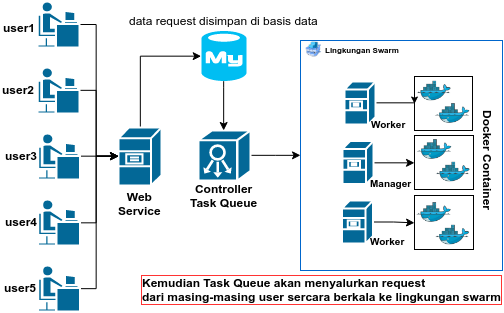
\includegraphics[width=10cm,height=7cm]{Images/C-5/taskqueue.png}
				\caption{Uji fungsionalitas penggunaan \textit{task queue} terhadap \textit{request user}}
				\label{gambartaskqueue}
			\end{figure}
			Uji coba ini dilakukan dengan cara menjalankan \textit{script} yang menggunakan bahasa pemrograman \textit{Python} pada \textit{crontab} yang ada di \textit{linux} dan dijadwalkan setiap 1 menit. Setiap kali pengguna mengirim \textit{request} uji beban melalui web, akan disimpan di basis data \textit{MySQL}. Ketika ada daftar antrian yang ada di basis data \textit{MySQL}, \textit{script} akan mengeksekusi hanya satu \textit{request} yang memiliki \textit{timestamp} paling awal dari beberapa \textit{request} yang lain dan akan dilakukan pengujian terhadap skenario yang dikirim. Setelah pengujian skenario selesai, status akan diubah menjadi \textit{done} dan \textit{script} akan mengeksekusi \textit{request} yang lain satu-persatu. Pada pengujian ini akan dilakukan oleh 5 pengguna yang akan melakukan \textit{request} uji beban. Gambaran pengujian ditunjukkan pada Gambar \ref{gambartaskqueue}.
			
		
		\subsubsection{Uji Fungsionalitas Pengambil Data Uji Beban}
			Uji coba ini dilakukan dengan cara menjalankan \textit{script puppeteer} pada setiap kontainer. \textit{script puppeteer} akan dijalankan ketika ada \textit{request} dari pengguna melalui \textit{web service} yang disediakan sistem. Gambaran pengujian ditunjukkan pada Gambar \ref{ambilhasiluji}.
			\begin{figure}[H]
				\centering
				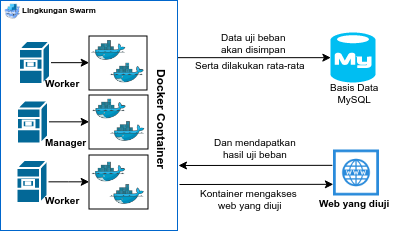
\includegraphics[width=9cm,height=6cm]{Images/C-5/ambilhasiluji.png}
				\caption{Uji fungsionalitas pengambil data uji beban}
				\label{ambilhasiluji}
			\end{figure}
		
		\subsubsection{Uji Fungsionalitas \textit{User} Melihat Hasil Uji Beban}
			Uji coba ini dilakukan dengan mengakses sistem melalui rute \texttt{/hasil}. Pengguna akan mengirimkan \textit{http request} kepada \textit{web service} yang telah disediakan. Rancangan pengujian dan hasil yang diharapkan ditunjukkan pada Tabel \ref{tabelujihasil}.
			\begin{longtable}{|p{0.05\textwidth}|p{0.25\textwidth}|p{0.30\textwidth}|p{0.30\textwidth}|}
				\caption{Skenario uji fungsionalitas \textit{user} melihat hasil uji beban} \label{tabelujihasil} \\ \hline
				\textbf{No} & \textbf{Rute} & \textbf{Uji Coba} & \textbf{Harapan} \\ \hline
				\endhead
				\endfoot
				\endlastfoot
				1 & /hasil/rata-rata & Mengirimkan \textit{request} menuju rute \textit{web service} melalui \textit{browser} & \textit{Request} berhasil diterima oleh \textit{web service}, kemudian \textit{web service} menampilkan hasil perhitungan rata-rata untuk hasil uji beban \\ \hline
				2 & /hasil/error-console & Mengirimkan \textit{request} menuju rute \textit{web service} melalui \textit{browser} & \textit{Request} berhasil diterima oleh \textit{web service}, kemudian \textit{web service} menampilkan daftar \textit{error console} yang terekam pada \textit{browser} \\ \hline
				3 & /hasil/images & Mengirimkan \textit{request} menuju rute \textit{web service} melalui \textit{browser} & \textit{Request} berhasil diterima oleh \textit{web service}, kemudian \textit{web service} menampilkan hasil tangkapan layar web yang diuji pada \textit{browser} \\ \hline
			\end{longtable}
		
	\subsection{Skenario Uji Performa} \label{skenujiperforma}
		Sistem \textit{load generator} dan pengambil data uji beban dibangun pada 3 buah \textit{node host} yang terpasang di lingkungan \textit{swarm}.  Sebelum dilakukan uji performa, dilakukan pemasangan \textit{load generator} yang diinisiasi pada terminal \textit{manager node}, kemudian \textit{manager node} akan mendistribusikan kontainer ke setiap \textit{node host} yang tergabung. Setelah selesai, data dari setiap kontainer akan disimpan di basis data. Uji coba akan dilakukan secara bertahap untuk membuat 500 kontainer, status awal kontainer sebelum diberikan \textit{request} akan \textit{sleep}. Setelah itu uji coba performa dilakukan untuk menguji performa sistem terhadap jumlah \textit{load generator} yang dikirimkan oleh pengguna. Pengujian akan dikirimkan oleh pengguna melalui \textit{web service} yang disediakan sistem. Jumlah \textit{load generator} yang akan diuji mulai dari 100, 200, 300, 400 dan 500. Hasil yang diharapkan dari pengujian performa sistem yaitu \textit{CPU} dan \textit{Memory} yang digunakan pada setiap \textit{node host}. Arsitektur pengujian tertera pada Gambar \ref{ujiperforma}.
		\begin{figure}[H]
			\centering
			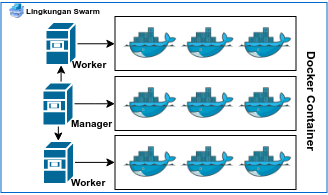
\includegraphics[width=9cm,height=6cm]{Images/C-5/performa.png}
			\caption{Arsitektur uji performa}
			\label{ujiperforma}
		\end{figure}
	
	\section{Hasil Uji Coba dan Evaluasi}
		Berikut dijelaskan hasil uji coba dan evaluasi berdasarkan skenario yang sudah dijelaskan pada bab \ref{skenarioujicoba}.
		
		\subsection{Uji Fungsionalitas}
			Berikut dijelaskan hasil pengujian fungsionalitas pada sistem yang sudah dibangun.
			
			\subsubsection{Uji Fungsionalitas \textit{User} Mengelola Skenario}
				Uji coba ini dilakukan dengan mengakses sistem melalui rute yang telah ditentukan pada Tabel \ref{tabelujiskenario}. Pengguna akan mengirim http request kepada web service yang telah
				disediakan. Hasil uji coba seperti tertera pada Tabel \ref{tabelhasilujiskenario}.
				\begin{longtable}{|p{0.05\textwidth}|p{0.25\textwidth}|p{0.40\textwidth}|p{0.12 \textwidth}|}
					\caption{Skenario uji fungsionalitas \textit{user} mengelola skenario} \label{tabelhasilujiskenario} \\ \hline
					\textbf{No} & \textbf{Rute} & \textbf{Harapan} & \textbf{Hasil} \\ \hline
					\endhead
					\endfoot
					\endlastfoot
					1 & /skenario & \textit{Request} berhasil diterima oleh \textit{web service}, kemudian \textit{web service} mengirimkan umpan balik berupa data skenario dari pengguna yang ditampilkan di \textit{browser} & OK \\ \hline
					2 & /skenario/create & \textit{Request} berhasil diterima oleh \textit{web service} dan halaman untuk membuat skenario ditampilkan di \textit{browser}  & OK \\ \hline
					3 & /skenario & \textit{Web service} berhasil menyimpan data skenario di basis data dan di setiap \textit{node host} dalam bentuk file konfig & OK \\ \hline
					4 & /skenario/\{id\} &\textit{Web service} berhasil menghapus data skenario di basis data dan di setiap \textit{node host} & OK \\ \hline
				\end{longtable}
				
			\subsubsection{Uji Fungsionalitas \textit{User} Mengirim Request Uji Beban}
				Uji coba ini dilakukan dengan mengakses sistem melalui rute yang telah ditentukan pada Tabel \ref{tabelujirequest}. Pengguna akan mengirim http request kepada web service yang telah
				disediakan. Hasil uji coba seperti tertera pada Tabel \ref{tabelhasilujirequest}.
				\begin{longtable}{|p{0.05\textwidth}|p{0.25\textwidth}|p{0.40\textwidth}|p{0.12 \textwidth}|}
					\caption{Skenario uji fungsionalitas \textit{user} mengirim request uji beban} \label{tabelhasilujirequest} \\ \hline
					\textbf{No} & \textbf{Rute} & \textbf{Harapan} & \textbf{Hasil} \\ \hline
					\endhead
					\endfoot
					\endlastfoot
					1 & /worker & \textit{Request} berhasil diterima oleh \textit{web service}, kemudian \textit{web service} menampilkan halaman untuk mengatur jumlah \textit{worker(load generator)} di \textit{browser} & OK \\ \hline
					2 & /worker & \textit{Web service} berhasil menyimpan data \textit{worker} dan membuat antrian \textit{request} di dalam basis data & OK \\ \hline
				\end{longtable}
				
			\subsubsection{Uji Fungsionalitas Penggunaan \textit{Task Queue} Terhadap \textit{Request User}}
				Uji coba ini akan dilakukan oleh 5 user yang melakukan request uji beban melalui \textit{web service} sesuai dengan penjelasan pada bab \ref{quuuueue}. Keterangan hasil uji yang dilakukan bisa dilihat pada Tabel \ref{quuuuueee}.
				\begin{longtable}{|p{0.15\textwidth}|p{0.12\textwidth}|p{0.35\textwidth}|p{0.18\textwidth}|p{0.10\textwidth}|}
					\caption{Hasil penggunaan \textit{task queue} terhadap \textit{request user}} \label{quuuuueee} \\
					\hline
					\textbf{Username} & \textbf{Jumlah} & \textbf{Link} & \textbf{Antrian ke} & \textbf{Hasil} \\ \hline
					\endhead
					\endfoot
					\endlastfoot
					user1 & 100 & https://dev.ppdbsda.net & 1 & OK \\ \hline
					user2 & 200 & https://dev.ppdbsda.net & 2 & OK \\ \hline
					user3 & 300 & https://dev.ppdbsda.net & 3 & OK \\ \hline
					user4 & 400 & https://dev.ppdbsda.net & 4 & OK \\ \hline
					user5 & 500 & https://dev.ppdbsda.net & 5 & OK \\ \hline
				\end{longtable}
				
			\subsubsection{Uji Fungsionalitas Pengambil Data Uji Beban}
				Uji coba ini akan dilakukan oleh \textit{Puppeteer} yang terpasang pada \textit{node host} di lingkungan \textit{swarm}. Skenario pengambil data uji beban sesuai dengan \textit{request task queue} pada Tabel \ref{quuuuueee}. Hasil dari pengujian ini dapat dilihat pada Tabel \ref{dataujibeban}.
				\begin{longtable}{|p{0.15\textwidth}|p{0.15\textwidth}|p{0.12\textwidth}|p{0.15\textwidth}|p{0.18\textwidth}|p{0.13\textwidth}|}
					\caption{Hasil pengambil data uji beban} \label{dataujibeban} \\
					\hline
					\textbf{Username} & \textbf{Response End} & \textbf{CSS Tracing End} & \textbf{DOM Content Loaded} & \textbf{First Meaningful Paint} & \textbf{Load Event End} \\ \hline
					\endhead
					\endfoot
					\endlastfoot
					user1 & 499,17 & 652,53 & 1592,35 & 1636,69 & 2001,26 \\ \hline
					user2 & 503,88 & 655,09 & 1589,95 & 1660,26 & 2010,12 \\ \hline
					user3 & 510,26 & 660,09 & 1567,26 & 1690,82 & 2084,83 \\ \hline
					user4 & 519,98 & 661,13 & 1598,62 & 1699,87 & 2188,10 \\ \hline
					user5 & 523,56 & 665,61 & 1599,40 & 1685,76 & 2190,45 \\ \hline
				\end{longtable}
			
				Selain itu akan didapatkan perhitungan presentase \textit{error} ketika terjadinya \textit{timeout} saat mengakses web yang diuji atau hasil \textit{performance metrics} pada Tabel \ref{dataujibeban} terdapat hasil kurang dari 0 atau minus.
				
			\subsubsection{Uji Fungsionalitas \textit{User} Melihat Hasil Uji Beban}
				Uji coba ini dilakukan dengan mengakses sistem melalui rute yang telah ditentukan pada Tabel \ref{tabelujihasil}. Pengguna akan mengirim \textit{http request} kepada \textit{web service} yang telah
				disediakan. Hasil uji coba seperti tertera pada Tabel \ref{tabelhasilujihasil}.
				\begin{longtable}{|p{0.05\textwidth}|p{0.25\textwidth}|p{0.40\textwidth}|p{0.12 \textwidth}|}
					\caption{Skenario uji fungsionalitas \textit{user} melihat hasil uji beban} \label{tabelhasilujihasil} \\ \hline
					\textbf{No} & \textbf{Rute} & \textbf{Uji Coba} & \textbf{Hasil} \\ \hline
					\endhead
					\endfoot
					\endlastfoot
					1 & /hasil/rata-rata & \textit{Request} berhasil diterima oleh \textit{web service}, kemudian \textit{web service} menampilkan hasil perhitungan rata-rata untuk hasil uji beban & OK \\ \hline
					2 & /hasil/error-console & \textit{Request} berhasil diterima oleh \textit{web service}, kemudian \textit{web service} menampilkan daftar \textit{error console} yang terekam pada \textit{browser} & OK \\ \hline
					3 & /hasil/images & \textit{Request} berhasil diterima oleh \textit{web service}, kemudian \textit{web service} menampilkan hasil tangkapan layar web yang diuji pada \textit{browser} & OK \\ \hline
				\end{longtable}
				

		\subsection{Uji Performa}
			Pengujian performa akan dilakukan pada 3 \textit{node host} yang ada di lingkungan \textit{swarm}. Pertama akan dilakukan pembuatan \textit{load generator(worker)}, kemudian akan dilakukan uji performa sistem ketika menerima request layanan uji beban.
			
			\subsubsection{Uji Pembuatan \textit{Load Generator}}
				Kondisi awal ketersediaan sumberdaya sebelum dilakukan pembuatan \textit{load generator} pada masing-masing \textit{node host} ditunjukkan pada Tabel \ref{suberdayaawalpembuatan}.
				\begin{longtable}{|p{0.05\textwidth}|p{0.25\textwidth}|p{0.14\textwidth}|p{0.17\textwidth}|p{0.14\textwidth}|}
					\caption{Kondisi awal ketersediaan sumberdaya sebelum pembuatan} \label{suberdayaawalpembuatan} \\
					\hline
					\textbf{No} & \textbf{Hostname} & \textbf{CPU} & \textbf{RAM} & \textbf{Storage} \\ \hline
					\endhead
					\endfoot
					\endlastfoot
					1 & CLOUD & 99,70\% & 287M/3.9G & 74/78G \\ \hline
					2 & RAIN & 99,64\% & 256M/3.9G & 74/78G \\ \hline
					3 & STORM & 99,69\% & 255M/3.9G & 74/78G \\ \hline
				\end{longtable}
			
				Setelah dilakukan uji coba untuk membuat kontainer yang akan digunakan sebagai \textit{load generator}, 
				ketersediaan sumberdaya \textit{CPU} dan \textit{RAM} ditunjukkan pada Tabel \ref{suberdayasetpembuatan} serta grafik  kondisi ketersediaan \textit{CPU} setelah pemasangan pada Gambar \ref{pembuatancpu} dan kondisi ketersediaan \textit{RAM} setelah pemasangan pada Gambar \ref{pembuatanram}.
				
				\begin{figure}[H]
					\centering
					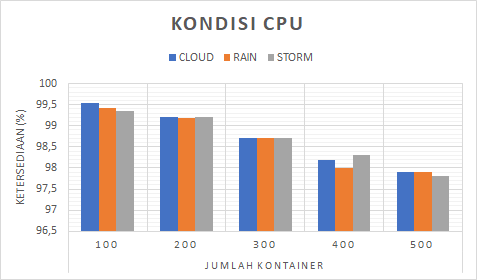
\includegraphics[width=8cm,height=5cm]{Images/C-5/pembuatancpu.png}
					\caption{Kondisi ketersediaan sumberdaya \textit{CPU} setelah pembuatan}
					\label{pembuatancpu}
				\end{figure}
				
				\begin{figure}[H]
					\centering
					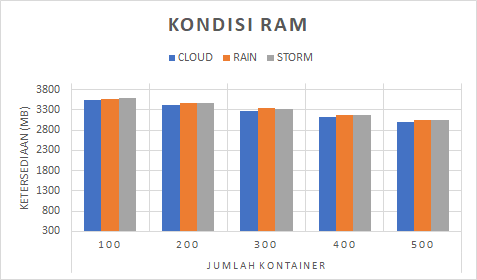
\includegraphics[width=8cm,height=5cm]{Images/C-5/pembuatanram.png}
					\caption{Kondisi ketersediaan sumberdaya \textit{RAM} setelah pembuatan}
					\label{pembuatanram}
				\end{figure}
			
				\begin{longtable}{|p{0.05\textwidth}|p{0.25\textwidth}|p{0.14\textwidth}|p{0.17\textwidth}|}
					\caption{Kondisi ketersediaan sumberdaya setelah pembuatan} \label{suberdayasetpembuatan} \\
					\hline
					\textbf{No} & \textbf{Hostname} & \textbf{CPU} & \textbf{RAM} \\ \hline
					\endhead
					\endfoot
					\endlastfoot
					1 & CLOUD & 97,9\% & 950M/3,9G \\ \hline
					2 & RAIN & 97,9\% & 892M/3,9G \\ \hline
					3 & STORM & 97,8\% & 889M/3,9G \\ \hline
				\end{longtable}
				
				Dari grafik tersebut dapat dilihat kebutuhan sumberdaya \textit{CPU} dan \textit{RAM} tidak mengalami perbedaan yang banyak dan hanya berubah secara \textit{linear}. \textit{CPU} tidak terlalu banyak berubah setelah pembuatan load generator dikarenakan semua \textit{load generator} di atur untuk \textit{sleep} sebelum ada \textit{request} uji beban. Namun ketika pembuatan \textit{load generator} dan pendistribusiannya, tentu saja penggunaan \textit{CPU} bisa sampai 100\% dan untuk kebutuhan sumberdaya \textit{RAM} adalah 1,3MB untuk setiap kontainernya. Pada tugas akhir ini, server yang digunakan hanya memiliki spesifikasi 2 \textit{Core CPU}. Adapun masalah-masalah yang dihadapi dalam pengujian ini yaitu ketika membuat \textit{load generator} dengan jumlah diatas 500 secara bersamaan yang akan mengakibatkan \textit{CPU Usage} bisa melebihi kapasitasnya dan hal tersebut akan membuat server \textit{not responding}.
				
				Sedangkan hasil distribusi kontainer ke setiap \textit{node host} setelah dilakukan pembuatan \textit{load generator} ditunjukkan pada Tabel \ref{jumlahkontainerpem}.
				\begin{longtable}{|p{0.05\textwidth}|p{0.30\textwidth}|p{0.15\textwidth}|p{0.15\textwidth}|p{0.15\textwidth}|}
					\caption{Hasil distribusi kontainer setelah pembuatan} \label{jumlahkontainerpem} \\
					\hline
					\textbf{No} & \textbf{Jumlah Kontainer} & \textbf{CLOUD} & \textbf{RAIN} & \textbf{STORM} \\ \hline
					\endhead
					\endfoot
					\endlastfoot
					1 & 100 & 34 & 33 & 33 \\ \hline
					2 & 200 & 66 & 67 & 67 \\ \hline
					3 & 300 & 100 & 100 & 100 \\ \hline
					4 & 400 & 132 & 134 & 134 \\ \hline
					5 & 500 & 166 & 167 & 167 \\ \hline
				\end{longtable}
			
				Pendistribusian pada Tabel \ref{jumlahkontainerpem} diatasi oleh manajer pada Docker Swarm dan didistribusikan secara rata ke setiap node host yang tergabung.
			
			\subsubsection{Uji Performa Sistem ketika Menerima Request Layanan Uji Beban}
%				Kondisi awal ketersediaan sumberdaya sebelum ada \textit{request} jumlah \textit{load generator} dari pengguna pada masing-masing \textit{node host} ditunjukkan pada Tabel \ref{suberdayaawalperforma}.
%				\begin{longtable}{|p{0.05\textwidth}|p{0.25\textwidth}|p{0.14\textwidth}|p{0.17\textwidth}|}
%					\caption{Kondisi awal ketersediaan sumberdaya sebelum pembuatan} \label{suberdayaawalperforma} \\
%					\hline
%					\textbf{No} & \textbf{Hostname} & \textbf{CPU} & \textbf{RAM} \\ \hline
%					\endhead
%					\endfoot
%					\endlastfoot
%					1 & CLOUD & 97,9\% & 950M/3,9G \\ \hline
%					2 & RAIN & 97,9\% & 892M/3,9G \\ \hline
%					3 & STORM & 97,8\% & 889M/3,9G \\ \hline
%				\end{longtable}
				
				Pengujian ini dilakukan ketika sistem menerima request layanan uji beban, informasi penggunaan sumberdaya ditunjukkan pada Tabel \ref{sdhasilperforma}, dari tabel tersebut didapatkan grafik penggunaan CPU pada Gambar \ref{performacpu} dan grafik penggunaan RAM pada Gambar \ref{performaram}.
				\begin{longtable}{|p{0.05\textwidth}|p{0.18\textwidth}|p{0.12\textwidth}|p{0.10\textwidth}|p{0.2\textwidth}|}
					\caption{Kondisi penggunaan sumberdaya ketika ada \textit{request}} \label{sdhasilperforma} \\
					\hline
					\textbf{No} & \textbf{Hostname} & \textbf{Jumlah} & \textbf{CPU} & \textbf{RAM} \\ \hline
					\endhead
					\endfoot
					\endlastfoot
					1 & CLOUD & 100 & 39,5\% & 1,1/3,9G \\ \cline{3-5}
					&& 200 & 52\% & 1,2/3,9G \\ \cline{3-5}
					&& 300 & 42,2\% & 1,3/3,9G \\ \cline{3-5}
					&& 400 & 48,7\% & 1,36/3,9G \\ \cline{3-5}
					&& 500 & 50,9\% & 1,39/3,9G \\ \hline
					2 & RAIN & 100 & 36,7\% & 1,02/3,9G \\ \cline{3-5}
					&& 200 & 46\% & 1,18/3,9G \\ \cline{3-5}
					&& 300 & 44,9\% & 1,3/3,9G \\ \cline{3-5}
					&& 400 & 46,8\% & 1,33/3,9G \\ \cline{3-5}
					&& 500 & 49\% & 1,4/3,9G \\ \hline
					3 & STORM & 100 & 38,9\% & 1,05/3,9G \\ \cline{3-5}
					&& 200 & 23\% & 1,12/3,9G \\ \cline{3-5}
					&& 300 & 40,2\% & 1,19/3,9G \\ \cline{3-5}
					&& 400 & 44,9\% & 1,38/3,9G \\ \cline{3-5}
					&& 500 & 49,6\% & 1,45/3,9G \\ \hline
				\end{longtable}
			
				\begin{figure}[H]
					\centering
					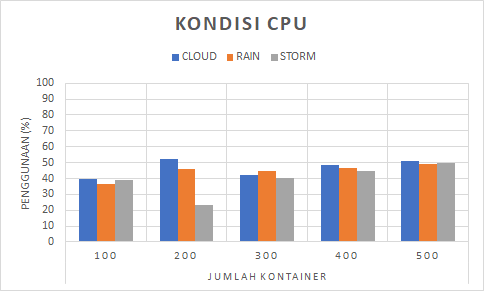
\includegraphics[width=8cm,height=5cm]{Images/C-5/performacpu.png}
					\caption{Kondisi penggunaan sumberdaya \textit{CPU} ketika ada \textit{request}}
					\label{performacpu}
				\end{figure}
			
				\begin{figure}[H]
					\centering
					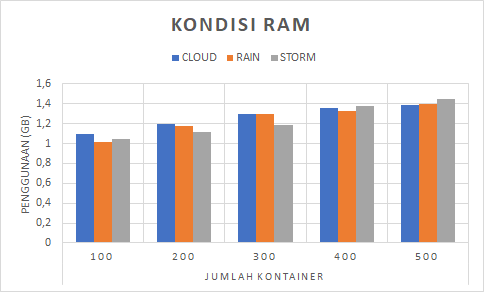
\includegraphics[width=8cm,height=5cm]{Images/C-5/performaram.png}
					\caption{Kondisi penggunaan sumberdaya \textit{RAM} ketika ada \textit{request}}
					\label{performaram}
				\end{figure}
			
				Berdasarkan grafik pada Gambar \ref{performacpu}, penggunaan \textit{CPU} mengalami perubahan secara \textit{linear} yaitu semakin banyak \textit{request} uji beban akan semakin tinggi, namun pada saat pengujian ketika jumlah \textit{load generator} 200, terjadi anomali pada ketersediaan sumberdaya, hal tersebut dikarenakan urutan kontainer id yang disimpan pada basis data tidak berimbang untuk nomor urut dari 1 sampai 200, sehingga pada \textit{node host} CLOUD dan RAIN memiliki jumlah \textit{load generator} yang harus dijalankan jauh lebih banyak dari pada \textit{node host} STORM, sehingga mengakibatkan tenjadinya anomali penggunaan \textit{CPU} pada \textit{node host} STORM.
				
				\indent Sedangkan untuk penggunaan \textit{RAM} pada Gambar \ref{performaram}, perubahannya secara linear saja, dikarenakan memang adanya pembatasan berjalannya proses secara bersama dalam setiap waktunya, karena \textit{Chrome} yang dijalankan akan memerlukan sumberdaya yang banyak. Jika tidak dibatasi, dapat mengakibatkan penggunaan \textit{CPU} dan \textit{RAM} akan melebihi kapasitas dan mengakibatkan server menjadi \textit{not responding}. Dapat dilihat dari kedua grafik, untuk penggunaan CPU sekitar 30-55\% dan RAM 1-1,4GB dalam melakukan uji beban karena dibatasi tersebut, namun ketika tidak adanya batasan, ketika menggunakan \textit{Headless Chrome} akan membutuhkan banyak sumberdaya \textit{CPU} dan \textit{RAM}, sedangkan untuk penggunaan \textit{Docker} relatif kecil dan tidak memerlukan sumberdaya sebanyak \textit{Headless Chrome}.
				
	\chapter{PENUTUP}
    Bab ini membahas kesimpulan yang dapat diambil dari tujuan pembuatan sistem dan hubungannya dengan hasil uji coba dan evaluasi yang telah dilakukan. Selain itu, terdapat beberapa saran yang bisa dijadikan acuan untuk melakukan pengembangan dan penelitian lebih lanjut.
        
	\section{Kesimpulan}
        Dari proses perencangan, implementasi dan pengujian terhadap sistem, dapat diambil beberapa kesimpulan berikut:
        \begin{enumerate}
        	\item Dalam pengembangan web, uji beban dapat dilakukan menggunakan \textit{Headless Chrome} sebagai \textit{tester}, yang dipadukan dengan \textit{API} pengambil uji beban yaitu \textit{Puppeteer}.
     		\item Load generator yang digunakan sebagai resource user dapat diimplementasikan oleh Docker. Docker dipasang menggunakan Docker Image yang sudah diinstalasi \textit{Node.js} dan \textit{Puppeteer} didalamnya.
        	\item Data Laporan uji beban didapatkan menggunakan \textit{Puppeteer} dan disajikan pada web dalam bentuk tabel dengan data inti yaitu \textit{Response End}, \textit{CSS Tracing End}, \textit{Dom Content Loaded}, \textit{First Meaningful Paint} dan \textit{Load Event End}. Laporan yang disajikan juga menampilkan \textit{error console} yang terekam pada \textit{browser} dan tangkapan layar web yang diuji.
        	\item Dalam menangani layanan uji beban yang dikirimkan oleh pengembang web, sistem menggunakan sebuah \textit{task scheduler crontab} yang menjalankan \textit{script Python} setiap satu menit dan melakukan pengecekan secara berkala.
        \end{enumerate}
        
	\section{Saran}
		Berikut beberapa saran yang diberikan untuk pengembangan lebih lanjut:
		\begin{itemize}
			\item Melakukan optimasi terhadap penggunaan \textit{CPU} dan \textit{RAM} supaya hasil uji lebih baik, misalnya menggunakan \textit{multithreading} untuk mengatur proses ketika dijalankan.
			\item Memadukan \textit{Headless Chrome} dan \textit{Puppeteer} dengan \textit{tools load test} yang lain misalnya \textit{K6}, \textit{Jmeter Rest API}, \textit{Selenium Web Driver} atau \textit{Firefox Headless Mode} untuk mendapatkan data uji beban.
			\item Untuk menangani permintaan jumlah \textit{load generator} yang tinggi, server yang digunakan harus dilakukan \textit{scaling} secara horizontal maupun vertikal, supaya dapat menunjang sistem untuk melayani uji beban.
			\item Pengembang bisa mempercantik tampilan antarmuka pengguna agar lebih nyaman untuk digunakan dan mengoptimasi layanan uji beban pada metode \textit{POST}.
		\end{itemize}

	\bibliography{Zotero}
	\bibliographystyle{IEEEtranID.bst}
    
    \renewcommand\chaptername{LAMPIRAN}
	\appendix
    \chapter{INSTALASI PERANGKAT LUNAK}

\section*{Instalasi \textit{Docker}}
	Untuk melakukan instalasi \textit{Docker}, dilakukan seperti langkah-langkah berikut:
\begin{lstlisting}[frame=single,tabsize=2,breaklines,caption={Perintah instalasi Docker },label=instalasidocker, captionpos=b, language=json,numbers=none]
$ sudo apt-get -y install \
apt-transport-https \
ca-certificates \
curl

$ curl -fsSL https://download.docker.com/linux/
ubuntu/gpg | sudo apt-key add -

$ sudo add-apt-repository \
"deb [arch=amd64] https://download.docker.com/linux/ubuntu \
$(lsb_release -cs) \
stable"

$ sudo apt-get update

$ sudo apt-get install docker-ce docker-ce-cli containerd.io
\end{lstlisting}
	
	Setelah menjalankan perintah pada kode sumber \ref{instalasidocker}. Jalankan perintah berikut agar \textit{Docker} bisa dijalankan sebagai \textit{Non-Root User}.
\begin{lstlisting}[frame=single,tabsize=2,breaklines,caption={Perintah mengubah hak User },label=nonrootuser, captionpos=b, language=json,numbers=none]
$ sudo groupadd docker
$ sudo usermod -aG docker $USER
\end{lstlisting}

\section*{Instalasi \textit{Docker Compose}}
\textit{Docker Compose} digunakan untuk otomasi dalam menjalankan \textit{Dockerfile} dan berperan untuk pembuatan Docker Image. Instalasi \textit{Docker Compose} dapat dilihat pada kode sumber \ref{dockercomposeinstall}.

\begin{lstlisting}[frame=single,tabsize=2,breaklines,caption={Perintah instalasi Docker Compose},label=dockercomposeinstall, captionpos=b, language=json,numbers=none]
$ sudo curl -L "https://github.com/docker/compose/releases/download/1.24.0/docker-compose-$(uname -s)-$(uname -m)" -o /usr/local/bin/docker-compose

$ sudo chmod +x /usr/local/bin/docker-compose

$ sudo ln -s /usr/local/bin/docker-compose /usr/bin/docker-compose
\end{lstlisting}

\section*{Instalasi \textit{Linux Package}}
Beberapa \textit{package} yang dibutuhkan dalam pembuatan sistem.
\begin{itemize}
	\item Node.js \\
		\texttt{\$ sudo apt install nodejs}\\
	\item NPM \\
		\texttt{\$ sudo apt install npm}\\
	\item MySQL \\
		\texttt{\$ sudo apt install mysql-server mysql-client}\\
	\item PIP \\
		\texttt{\$ sudo apt install python3-pip}\\
	\item mysql-connector-python \\
		\texttt{\$ pip3 install mysql-connector-python}\\
	\item Composer \\
		\texttt{\$ php -r "copy('https://getcomposer.org/installer', 'composer-setup.php');"} \\ \\
		\texttt{\$ php -r "if (hash\_file('sha384', 'composer-setup.php') === '48e3236262b34d30969dca3c37281b3b4bbe3221bda826ac6a9a62d6444cdb0dcd0615698a5cbe587c3f0fe57a54d8f5') { echo 'Installer verified'; } else { echo 'Installer corrupt'; unlink('composer-setup.php'); } echo PHP\_EOL;"}\\ \\
		\texttt{\$ php composer-setup.php} \\
		\texttt{\$ php -r "unlink('composer-setup.php');"} \\
		\texttt{\$ mv composer.phar /usr/local/bin/composer} \\
	\item Laravel \\
		\texttt{\$ composer global require laravel/installer}\\
\end{itemize}
    \chapter{KODE SUMBER}

\section*{Kode Sumber Pengambilan Data Metrics Performance} \label{puppeteer}
	\subsection*{Isi berkas index.js}
\begin{lstlisting}[frame=single,tabsize=2,breaklines,caption={Isi berkas index.js},label=indexjs, captionpos=b, language=json]
const puppeteer = require('puppeteer');
const testPage = require('./testPage');
const fs = require('fs');
const db = require('../config/databases');
const scenario_id = process.argv[2];
const counter = process.argv[3];
const worker = process.argv[4];
const host = process.argv[5];

let rawdata = fs.readFileSync('/app/code/assets/config_'+scenario_id+'.json');  
let config = JSON.parse(rawdata);
(async () => {
	const browser = await puppeteer.launch({args: ['--no-sandbox']});
	const page = await browser.newPage();
	await page.on('console', msg => 
		db.query('INSERT INTO errors (scenario_id, link, worker, username, host, type, text, location_url) VALUES (?, ?, ?, ?, ?, ?, ?, ?)', 
		[ scenario_id, config.scenario_link, worker, config.username, host, msg._type, msg._text, msg._location.url ])
	);
	try{
		let data = await testPage(page, config, counter);
		db.query('INSERT INTO tests (scenario_id, link, worker, username, host, response_end, dom_interactive, dom_content_load, load_event_end, css_trace_start, css_trace_end, first_meaningful, timestamp) VALUES (?, ?, ?, ?, ?, ?, ?, ?, ?, ?, ?, ?, ?)', 
		[ scenario_id, config.scenario_link, worker, config.username, host, data.Timing.responseEnd, data.Timing.domInteractive, data.Timing.domContentLoadedEventEnd, data.Timing.loadEventEnd, data.TraceResult.cssStart, data.TraceResult.cssEnd, data.Metrics.FirstMeaningfulPaint, data.Metrics.Timestamp ]);
		db.end();
		await page.screenshot({path: '/app/output/ss'+scenario_id+'.png'});
		await browser.close();
	} catch(error) {
		console.error(error);
		await page.screenshot({path: '/app/output/ss'+scenario_id+'.png'});
		await browser.close();
	}
})();
\end{lstlisting}

	\subsection*{Isi berkas testPage.js}
\begin{lstlisting}[frame=single,tabsize=2,breaklines,caption={Isi berkas testPage.js},label=testjs, captionpos=b, language=json]
const {
getTimeFromPerformanceMetrics,
	extractDataFromPerformanceMetrics,
	extractDataFromPerformanceTiming,
	extractDataFromTracing,
} = require('./helpers');

async function testPage(page, config, counter) {
	const client = await page.target().createCDPSession();
	await client.send('Performance.enable');
	const navigationStart = getTimeFromPerformanceMetrics(
		await client.send('Performance.getMetrics'),
		'NavigationStart'
	);
	
	await page.tracing.start({ path: './trace'+config.scenario_id+counter+'.json' });
	
	await page.goto(config.scenario_link);

	if(config.scenario_method == 'POST'){
		if(config.incr == 'true'){
			for(var i=0; i<config.attr.length; i++){
				await page.type('#'+config.attr[i], config.val_attr[i]+counter);
			}
			await page.click('button[type='+config.scenario_button+']');
		} else {
			for(var i=0; i<config.attr.length; i++){
				await page.type('#'+config.attr[i], config.val_attr[i]);
			}
			await page.click('button[type='+config.scenario_button+']');
		} 
	}

	const performanceTiming = JSON.parse(
		await page.evaluate(() => JSON.stringify(window.performance.timing))
	);

	let firstMeaningfulPaint = 0;
	while (firstMeaningfulPaint === 0) {
		await page.waitFor(300);
		performanceMetrics = await client.send('Performance.getMetrics');
		firstMeaningfulPaint = getTimeFromPerformanceMetrics(
			performanceMetrics, 'FirstMeaningfulPaint'
		);
	}

	await page.tracing.stop();

	const cssTracing = await extractDataFromTracing(
		'./trace'+config.scenario_id+counter+'.json',
		config.scenario_link,
	);

	let TraceResult = {
		cssStart: cssTracing.start - navigationStart,
		cssEnd: cssTracing.end - navigationStart,
	}

	let Metrics = extractDataFromPerformanceMetrics(
		performanceMetrics,
		'Timestamp',
		'FirstMeaningfulPaint',
	);

	let Timing = extractDataFromPerformanceTiming(
		performanceTiming,
		'responseEnd',
		'domInteractive',
		'domContentLoadedEventEnd',
		'loadEventEnd',
	);

	return { TraceResult, Metrics, Timing };
}

module.exports = testPage;
\end{lstlisting}

	\subsection*{Isi berkas helpers.js}
\begin{lstlisting}[frame=single,tabsize=2,breaklines,caption={Isi berkas helpers.js},label=helperjs, captionpos=b, language=json]
const fs = require('fs');

const getTimeFromPerformanceMetrics = (metrics, name) =>
	metrics.metrics.find(x => x.name === name).value * 1000;

const extractDataFromPerformanceMetrics = (metrics, ...dataNames) => {
	const navigationStart = getTimeFromPerformanceMetrics(
		metrics,
		'NavigationStart'
	);
	const extractedData = {};
	dataNames.forEach(name => {
		extractedData[name] =
			getTimeFromPerformanceMetrics(metrics, name) - navigationStart;
	});
	return extractedData;
};

const extractDataFromPerformanceTiming = (timing, ...dataNames) => {
	const navStart = timing.navigationStart;

	const extractedData = {};
	dataNames.forEach(name => {
		extractedData[name] = timing[name] - navStart;
	});

	return extractedData;
};

const extractDataFromTracing = (path, link) => new Promise(resolve => {
	const tracing = JSON.parse(fs.readFileSync(path, 'utf8'));
	const resourceTracings = tracing.traceEvents.filter(
		x =>
			x.cat === 'devtools.timeline' &&
			typeof x.args.data !== 'undefined' &&
			typeof x.args.data.url !== 'undefined' &&
			x.args.data.url.includes(link)
	);
	const resourceTracingSendRequest = resourceTracings.find(
		x => x.name === 'ResourceSendRequest'
	);
	const resourceId = resourceTracingSendRequest.args.data.requestId;
	const resourceTracingEnd = tracing.traceEvents.filter(
		x =>
			x.cat === 'devtools.timeline' &&
			typeof x.args.data !== 'undefined' &&
			typeof x.args.data.requestId !== 'undefined' &&
			x.args.data.requestId === resourceId
	);
	const resourceTracingStartTime = resourceTracingSendRequest.ts / 1000;
	const resourceTracingEndTime =
		resourceTracingEnd.find(x => x.name === 'ResourceFinish').ts / 1000;
	
	fs.unlink(path, () => {
		resolve({
			start: resourceTracingStartTime,
			end: resourceTracingEndTime,
		});
	});
});

module.exports = {
	getTimeFromPerformanceMetrics,
	extractDataFromPerformanceMetrics,
	extractDataFromPerformanceTiming,
	extractDataFromTracing,
};
\end{lstlisting}

\section*{Kode Sumber Basis Data MySQL} \label{mysql}
	
\begin{lstlisting}[frame=single,tabsize=2,breaklines,caption={Basis data MySQL},label=mysql, captionpos=b, language=json]
-- membuat tabel containers -> untuk menyimpan data kontainer
CREATE TABLE `containers` (
	`id` bigint(20) unsigned NOT NULL AUTO_INCREMENT,
	`task_id` varchar(255) COLLATE utf8mb4_unicode_ci NOT NULL,
	`node_id` varchar(255) COLLATE utf8mb4_unicode_ci NOT NULL,
	`container_id` varchar(255) COLLATE utf8mb4_unicode_ci NOT NULL,
	`node_ip` varchar(255) COLLATE utf8mb4_unicode_ci NOT NULL,
	`node_host` varchar(255) COLLATE utf8mb4_unicode_ci NOT NULL,
	`status` smallint(6) NOT NULL DEFAULT '0',
	`username` varchar(100) COLLATE utf8mb4_unicode_ci NOT NULL DEFAULT '0',
	PRIMARY KEY (`id`)
) ENGINE=InnoDB AUTO_INCREMENT=1 DEFAULT CHARSET=utf8mb4 COLLATE=utf8mb4_unicode_ci;

-- membuat tabel errors -> untuk menyimpan error console
CREATE TABLE `errors` (
	`id` bigint(20) unsigned NOT NULL AUTO_INCREMENT,
	`scenario_id` varchar(255) COLLATE utf8mb4_unicode_ci DEFAULT NULL,
	`link` varchar(255) COLLATE utf8mb4_unicode_ci DEFAULT NULL,
	`worker` varchar(255) COLLATE utf8mb4_unicode_ci DEFAULT NULL,
	`username` varchar(100) COLLATE utf8mb4_unicode_ci DEFAULT NULL,
	`host` varchar(100) COLLATE utf8mb4_unicode_ci DEFAULT NULL,
	`type` varchar(100) COLLATE utf8mb4_unicode_ci DEFAULT NULL,
	`text` varchar(255) COLLATE utf8mb4_unicode_ci DEFAULT NULL,
	`args` varchar(255) COLLATE utf8mb4_unicode_ci DEFAULT NULL,
	`location_url` varchar(255) COLLATE utf8mb4_unicode_ci DEFAULT NULL,
	PRIMARY KEY (`id`)
) ENGINE=InnoDB DEFAULT CHARSET=utf8mb4 COLLATE=utf8mb4_unicode_ci;

-- membuat tabel results -> untuk menyimpan hasil rata-rata perhitungan hasil pengujian
CREATE TABLE `results` (
	`id` bigint(20) unsigned NOT NULL AUTO_INCREMENT,
	`scenario_id` varchar(255) COLLATE utf8mb4_unicode_ci DEFAULT NULL,
	`link` varchar(255) COLLATE utf8mb4_unicode_ci DEFAULT NULL,
	`method` varchar(100) COLLATE utf8mb4_unicode_ci DEFAULT NULL,
	`worker` varchar(255) COLLATE utf8mb4_unicode_ci DEFAULT NULL,
	`username` varchar(100) COLLATE utf8mb4_unicode_ci DEFAULT NULL,
	`error` varchar(100) COLLATE utf8mb4_unicode_ci DEFAULT NULL,
	`response_end` varchar(100) COLLATE utf8mb4_unicode_ci DEFAULT NULL,
	`dom_interactive` varchar(100) COLLATE utf8mb4_unicode_ci DEFAULT NULL,
	`dom_content_load` varchar(100) COLLATE utf8mb4_unicode_ci DEFAULT NULL,
	`load_event_end` varchar(100) COLLATE utf8mb4_unicode_ci DEFAULT NULL,
	`css_trace_start` varchar(100) COLLATE utf8mb4_unicode_ci DEFAULT NULL,
	`css_trace_end` varchar(100) COLLATE utf8mb4_unicode_ci DEFAULT NULL,
	`first_meaningful` varchar(100) COLLATE utf8mb4_unicode_ci DEFAULT NULL,
	`timestamp` varchar(100) COLLATE utf8mb4_unicode_ci DEFAULT NULL,
	PRIMARY KEY (`id`)
) ENGINE=InnoDB DEFAULT CHARSET=utf8mb4 COLLATE=utf8mb4_unicode_ci;

-- membuat tabel scenarios -> untuk menyimpan scenario pengujian
CREATE TABLE `scenarios` (
	`id` bigint(20) unsigned NOT NULL AUTO_INCREMENT,
	`created_at` timestamp NULL DEFAULT NULL,
	`updated_at` timestamp NULL DEFAULT NULL,
	`scenario_id` varchar(255) COLLATE utf8mb4_unicode_ci NOT NULL,
	`username` varchar(255) COLLATE utf8mb4_unicode_ci NOT NULL,
	`scenario_method` varchar(255) COLLATE utf8mb4_unicode_ci NOT NULL,
	`scenario_link` varchar(255) COLLATE utf8mb4_unicode_ci NOT NULL,
	`scenario_worker` varchar(255) COLLATE utf8mb4_unicode_ci DEFAULT NULL,
	`scenario_status` smallint(6) DEFAULT '0',
	`scenario_button` varchar(100) COLLATE utf8mb4_unicode_ci DEFAULT NULL,
	PRIMARY KEY (`id`)
) ENGINE=InnoDB DEFAULT CHARSET=utf8mb4 COLLATE=utf8mb4_unicode_ci;

-- membuat tabel swarms -> untuk menyimpan swarm node
CREATE TABLE `swarms` (
	`id` bigint(20) unsigned NOT NULL AUTO_INCREMENT,
	`created_at` timestamp NULL DEFAULT NULL,
	`updated_at` timestamp NULL DEFAULT NULL,
	`swarm_ip` varchar(255) COLLATE utf8mb4_unicode_ci NOT NULL,
	`swarm_username` varchar(255) COLLATE utf8mb4_unicode_ci NOT NULL,
	`swarm_password` varchar(255) COLLATE utf8mb4_unicode_ci NOT NULL,
	`is_used` smallint(6) DEFAULT '0',
	PRIMARY KEY (`id`),
	UNIQUE KEY `swarms_swarm_ip_unique` (`swarm_ip`)
) ENGINE=InnoDB AUTO_INCREMENT=4 DEFAULT CHARSET=utf8mb4 COLLATE=utf8mb4_unicode_ci;

-- membuat tabel test -> untuk menyimpan hasil setiap pengujian
CREATE TABLE `tests` (
	`id` bigint(20) unsigned NOT NULL AUTO_INCREMENT,
	`scenario_id` varchar(255) COLLATE utf8mb4_unicode_ci DEFAULT NULL,
	`link` varchar(255) COLLATE utf8mb4_unicode_ci DEFAULT NULL,
	`worker` varchar(255) COLLATE utf8mb4_unicode_ci DEFAULT NULL,
	`username` varchar(100) COLLATE utf8mb4_unicode_ci DEFAULT NULL,
	`host` varchar(100) COLLATE utf8mb4_unicode_ci DEFAULT NULL,
	`response_end` varchar(100) COLLATE utf8mb4_unicode_ci DEFAULT NULL,
	`dom_interactive` varchar(100) COLLATE utf8mb4_unicode_ci DEFAULT NULL,
	`dom_content_load` varchar(100) COLLATE utf8mb4_unicode_ci DEFAULT NULL,
	`load_event_end` varchar(100) COLLATE utf8mb4_unicode_ci DEFAULT NULL,
	`css_trace_start` varchar(100) COLLATE utf8mb4_unicode_ci DEFAULT NULL,
	`css_trace_end` varchar(100) COLLATE utf8mb4_unicode_ci DEFAULT NULL,
	`first_meaningful` varchar(100) COLLATE utf8mb4_unicode_ci DEFAULT NULL,
	`timestamp` varchar(100) COLLATE utf8mb4_unicode_ci DEFAULT NULL,
	`status` smallint(6) DEFAULT '0',
	PRIMARY KEY (`id`)
) ENGINE=InnoDB DEFAULT CHARSET=utf8mb4 COLLATE=utf8mb4_unicode_ci;

-- membuat tabel users -> menyimpan user
CREATE TABLE `users` (
	`id` bigint(20) unsigned NOT NULL AUTO_INCREMENT,
	`name` varchar(255) COLLATE utf8mb4_unicode_ci NOT NULL,
	`email` varchar(255) COLLATE utf8mb4_unicode_ci NOT NULL,
	`username` varchar(255) COLLATE utf8mb4_unicode_ci NOT NULL,
	`email_verified_at` timestamp NULL DEFAULT NULL,
	`password` varchar(255) COLLATE utf8mb4_unicode_ci NOT NULL,
	`remember_token` varchar(100) COLLATE utf8mb4_unicode_ci DEFAULT NULL,
	`created_at` timestamp NULL DEFAULT NULL,
	`updated_at` timestamp NULL DEFAULT NULL,
	PRIMARY KEY (`id`),
	UNIQUE KEY `users_email_unique` (`email`),
	UNIQUE KEY `users_username_unique` (`username`)
) ENGINE=InnoDB AUTO_INCREMENT=3 DEFAULT CHARSET=utf8mb4 COLLATE=utf8mb4_unicode_ci;
\end{lstlisting}

	\appendix

	\backmatter % Lampiran tanpa judul LAMPIRAN X, biasanya untuk BIODATA PENULIS
	\chapter{BIODATA PENULIS}
	\begin{wrapfigure}{l}{0.3\textwidth}
		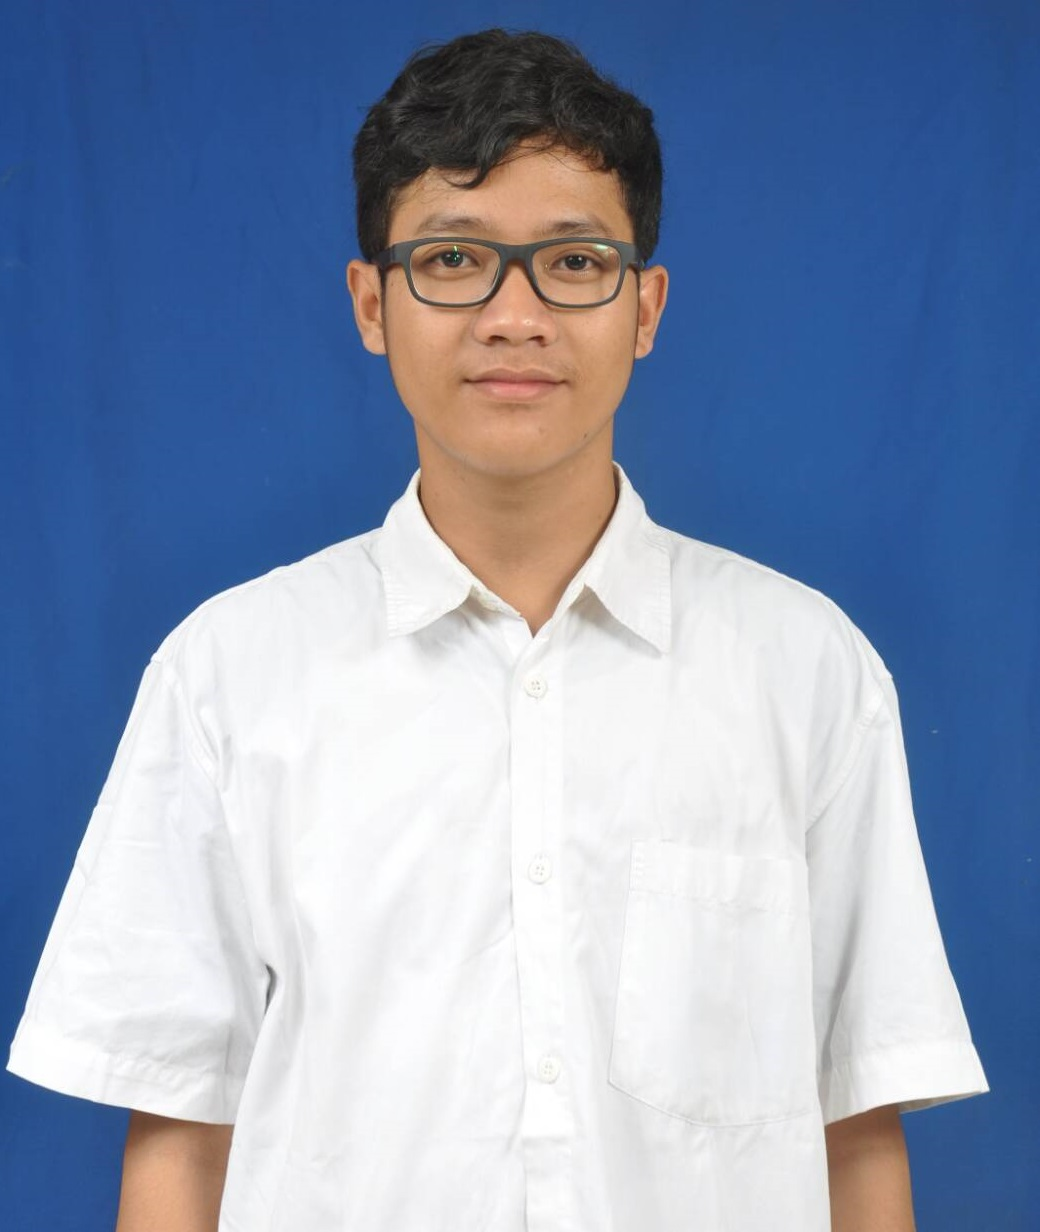
\includegraphics[width=0.29\textwidth]{img/CPH.jpg}
	\end{wrapfigure}
	
	\textbf{Cahya Putra Hikmawan}, biasa disapa Awan dan lahir pada tanggal 09 September 1996 di Krembung, Kabupaten Sidoarjo. Penulis telah menempuh pendidikan formal di SD Al-Ishlah, SMP Negeri 1 Krembung, MBI Amanatul Ummah Pacet dan melanjutkan studi program sarjana di Departemen Informatika, Institut Teknologi Sepuluh Nopember. Penulis memiliki hobi antara lain membaca novel, menonton drama dan memancing. Selama menempuh pendidikan di Departemen Informatika ITS, penulis aktif dalam kegiatan akademik dan non akademik. Di bidang akademik penulis pernah menjadi asisten dosen dan asisten praktikum untuk mata kuliah Sistem Operasi (2017 dan 2019), Jaringan Komputer (2017-2018), serta menjadi Koor Asisten Praktikum untuk mata kuliah Jaringan Komputer (2017). Selain itu penulis menjadi Admin Laboratorium Arsitektur dan Jaringan Komputer (AJK) dan mengikuti kegiatan pelatihan linux di tulungagung sebagai asisten dan panitia. Sedangkan untuk kegiatan non akademik penulis aktif  menjadi Staf dan Badan Pengurus Harian II NLC (National Logic Competition) Schematics 2016 dan Schematics 2017, Staf dan Staf Ahli Departemen Pengembangan Profesi Himpunan Mahasiswa Teknik Computer-Informatika (HMTC) ITS. Penulis dapat dihubungi melalui surat elektronik di \texttt{cp.hikmawan@gmail.com}.
\end{document}

\end{document} % Marii CUuuukkkk!! Alhamdulillah :)
